\documentclass[a4paper]{article}
 
\usepackage{enumitem}
%\usepackage[german]{babel}
\usepackage[utf8]{inputenc}
\usepackage[T1]{fontenc}
\usepackage{ae}
\usepackage[bookmarks,bookmarksnumbered]{hyperref}
\usepackage[toc]{glossaries}
\usepackage{graphicx}
\usepackage{wrapfig}
\usepackage{hyperref}
\usepackage{wrapfig}
\usepackage{fancyhdr}

%\usepackage[backend=bibtex,
%style=numeric
%%style=alphabetic
%%style=reading
%]{biblatex}
%\addbibresource{lit}

\setlength\parindent{5mm}

\graphicspath{ {img/} }

\pagestyle{fancy}
\fancyhead[L]{Votes - Electronic Polls Made Easy}
%\fancyhead[R]{\leftmark}


\begin{document}


\begin{titlepage}

\centering


{\Huge\fontsize{40}{40} \textbf{Votes}}
\\ \vspace*{7mm}
{\LARGE \textbf{- Electronic Polls Made Easy -}}
%{\huge \textbf{Handbook}}
\\ \vspace*{3mm}

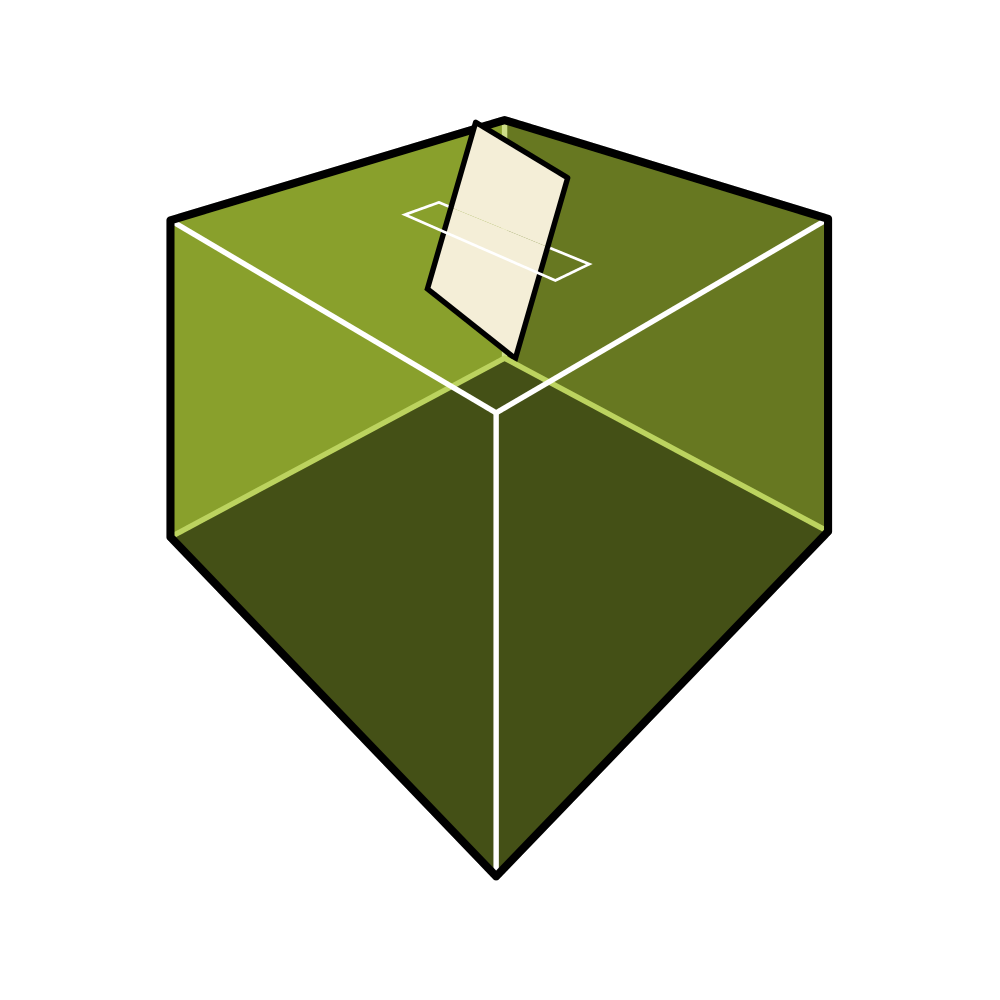
\includegraphics[width=\textwidth]{votes.png}

{\huge \textsc{University of Koblenz-Landau}}
\\ \vspace*{3mm}
{\Large \textsc{Summer Term 2014}}
\\ \vspace*{7mm}
{\large
Jan-Hendrik Borth,
Johannes Härtel,\\
Maximilian Meffert, 
Lukas Müller 
}

\end{titlepage}

\newpage
\vspace*{\fill}
\newpage
\vspace*{\fill}
\begin{center}
{\huge \textsc{Abstract}}
\\ \vspace*{7mm}
\begin{minipage}[m]{0.9\textwidth}
\large
\textsc{Votes - Electronic Polls Made Easy} is the examination project of the JavaEE course in summer semester 2014 at the University of Koblenz-Landau.
This document summarizes the initial challenge, the met requirements and elaborates the solution architecture.
Moreover, the document includes an installation guide for the proposed solution.
\end{minipage}
\end{center}
\vspace*{\fill}
\newpage
\tableofcontents
\newpage
\listoffigures
\newpage
\section{Introduction}
\textit{Votes - Electronic Polls Made Easy} is the examination project of the JavaEE course in summer semester 2014 at the University of Koblenz-Landau.
\section{Requirements}
\label{requirements}



In this section the requirements realised by the system are listed. The enumeration mirrors the requirement list defined in \cite{Votes14}. The identifications numbers are identical. Requirements that are not completely implemented are left out.

% TODO: remove MANDATORY... and add if realized. Maybe with short description.

\subsection{Functional Requirements}



\begin{enumerate}

\item[1.] Polls

	\begin{enumerate}
	\item
	[1.1.] The system must support electronic polls with one or more items. MANDATORY
	
	
	\item
	[1.2.] Each poll must have a title. The title has to be unique (scope is system). MANDATORY
	
	
	\item
	[1.3.] Each poll must have a description. MANDATORY
	
	
	\item
	[1.4.] Each poll must have a voting period (start and end date with time). MANDATORY
	
	
	\item
	[1.5.] Each poll must have at least one item. MANDATORY
	
	
	\item
	[1.6.] The system must allow to group arbitrary many items into one poll. MANDATORY
	
	\end{enumerate}




\item[2.] Poll states

	\begin{enumerate}
	\item
	[2.1.] The system must implement poll states. Polls be in one of four states: PREPARED, STARTED,
	VOTING, FINISHED. State changes are specified in figure \ref{figure:poll-states}. MANDATORY
	
	
	\item
	[2.2.] When all participants submitted their votes, the system must set the poll to FINISHED.
	MANDATORY
	
	
	\item
	[2.3.] An organizer must be able to extend the voting period when a poll is in state STARTED or
	VOTING. OPTIONAL
	\end{enumerate}




\item[3.] Organizers

	\begin{enumerate}
	\item
	[3.1.] The system must allow all university members to act as organizers. MANDATORY
	
	
	\item
	[3.2.] Organizers must identify themselves with username and password. MANDATORY
	
		\begin{enumerate}
		
		
		\item
		[3.2.1.] University members can be identified by the LDAP service provided by the GHRKO
		computing center. OPTIONAL
		
		
		\item
		[3.2.2.] If LDAP is not used, an administrator must be able to create organizer accounts. OPTIONAL
	
		\end{enumerate}
	
	
	
	
	\item
	[3.3.] An organizer must be able to conduct arbitrary many polls. MANDATORY
	
	
	\item
	[3.4.] The system shall provide a preview mode that allows organizers to view how their polls look
	like when a participant fills in her choices. OPTIONAL
	
	
	\item
	[3.5.] The system can provide a possibility to add further organizers to a poll. Each organizer must
	have the same options. OPTIONAL
	
		\begin{enumerate}
			\item[3.5.1.] An organizer must be able to change the organizer list.
			
			
			\item[3.5.2.] An organizer must not be able to remove herself from the organizer list.
		
		\end{enumerate}
	
	
	\end{enumerate}




\item[4.] Administrators

	\begin{enumerate}
	\item[4.1.] The system must support an administrator role. OPTIONAL
	
	
	\item[4.2.] Administrators must have the ability to delete polls (including all votes) from the system. OPTIONAL
	
	
	\item[4.3.] Administrators must not be able to view votes nor results of polls which they didn't organize.
	OPTIONAL
	
	
	\item[4.4.] Administrators must be able to create and delete user accounts, if no LDAP authentication is
	provided (see requirement XXX). OPTIONAL
	\end{enumerate}




\item[5.] Participants

	\begin{enumerate}
	\item[5.1.] The organizer of a poll must be able to invite 3 to arbitrary many participants. In polls with
	less than 3 participants, anonymity can not be asserted. MANDATORY
	
	
	\item[5.2.] Each participant must be identified by her email address. MANDATORY
	
	
	\item[5.3.] The system shall support participants from outside the university. OPTIONAL
	
	
	\item[5.4.] After a poll is STARTED by the organizer, each participant must be informed via email about
	the poll. OPTIONAL (University mail server must not be „mis-used“, it’s sufficient to display
	the mail content on a web page)
	
	
	\item[5.5.] The information mail must include the title of the poll, the start and end dates, the number of
	participants, and a token. MANDATORY
	
	
	\item[5.6.] The information can also contain a hyperlink immediately referring to the voting page with a
	pre-filled token field. OPTIONAL
	\end{enumerate}




\item[6.] Participant lists

	\begin{enumerate}
	\item[6.1.] The organizer must be able to modify the participant list until a poll is STARTED. MANDATORY
	
	
	\item[6.2.] The system can provide a means to comfortably create participant lists, e.g. by pasting
	email addresses from other applications such as spread sheets or KLIPS. OPTIONAL
	
	
	\item[6.3.] The system shall provide a means to store participant lists for easy reuse in subsequent
	polls. OPTIONAL
	
	
	\item[6.3.1.] The stored participant lists must be private to each organizer.
	
	
	\item[6.3.2.] Each stored participant list must have a unique name (scope is per organizer).
	\end{enumerate}





\item[7.] Tokens

	\begin{enumerate}
	\item[7.1.] The token must be randomly chosen. MANDATORY
	
	
	\item[7.2.] The token must be unique (scope is system). MANDATORY
	
	
	\item[7.3.] The token must be long enough to make it very very improbable that anybody can forge a
	valid token. MANDATORY
	\end{enumerate}




\item[8.] Anonymity

	\begin{enumerate}
	\item[8.1.] The system must ensure anonymity. MANDATORY (with reasonable effort)
	
	
	\item[8.2.] At any point in time it must be impossible to identify which participant submitted which vote.
	This also must to be guaranteed for polls with participation tracking. MANDATORY
	
	
	\item[8.3.] The system must ensure that a token can not be associated with a vote. MANDATORY
	\end{enumerate}



\item[9.] Participation tracking

	\begin{enumerate}
	\item[9.1.] The system must provide an option to enable participation tracking for a poll. OPTIONAL
	
	
	\item[9.2.] The system can provide an option to configure automatic reminders via E-Mail. OPTIONAL
	\end{enumerate}




\item[10.] Submitting a vote

	\begin{enumerate}
	\item[10.1.] The system must provide a web page to submit a vote. MANDATORY
	
	
	\item[10.2.] The voting page must present an input field for a participant’s token. MANDATORY
	
	
	\item[10.3.] The token input field can be pre-filled (see requirement XX). OPTIONAL
	
	
	\item[10.4.] After the token was verified, the system must display the items. MANDATORY
	
	
	\item[10.5.] The system must present a button to submit a vote. MANDATORY
	
	
	\item[10.6.] After a vote was submitted, the token used for that vote must be invalidated (i.e. it can’t be
	re-used, participants can not change their vote after submitting). MANDATORY
	
	
	\item[10.7.] The system must allow to cancel a voting (e.g. by closing the browser, or by clicking a cancel
	button). MANDATORY
	
	
	\item[10.8.] The token used in canceled voting must be re-useable later. MANDATORY
	
	
	\item[10.9.] For a canceled voting, the system must not remember any of the choices. OPTIONAL
	
	
	\item[10.10.] The system shall ensure that subsequent participants using the same browser window
	can not restore the previous choice (e.g. by the „go back“ function or by auto fill capabilities
	of browsers). OPTIONAL
	\end{enumerate}




\item[11.] Abstain from voting

	\begin{enumerate}
	\item[11.1.] The system must provide a means to abstain from voting (Enthaltung oder ungültige
	Stimme) for each item of a poll. MANDATORY
	
	
	\item[11.2.] The system can provide a means to abstain from voting for a complete poll (this is equivalent
	to abstaining from all items). OPTIONAL
	
	\end{enumerate}



\item[12.] Types of items

	\begin{enumerate}
	\item[12.1.] The system must support different types of items. MANDATORY
	
	
	\item[12.2.] The items of a poll must have a title (titles have to be unique with scope poll). MANDATORY
	
	
	\item[12.3.] The options of an item must have a short name and a description. MANDATORY
	
	
	\item[12.4.] The system must support YES/NO items. In this case, the short names of the options are
	„yes“ and „no“. MANDATORY
	
	
	\item[12.5.] The system must support 1 OF N items. Participants can choose exactly one of zwo or
	more options. MANDATORY
	
	
	\item[12.6.] The system must support M OF N items. Participants can choose at most M of two or
	more options (M $\leq$ N). OPTIONAL
	
	
	\item[12.7.] The system can support 1 OF N items with a free text option. Participants can choose one
	of the predefined options. Alternatively, they can enter a free text to indicate their choice.
	OPTIONAL
	
	
	\item[12.8.] The system can support M OF N items with up to M free text options. Participants can
	choose at most M of the predefined options. Alternatively, they can can use less than M
	predefined options an enter the rest of their choices into free text fields. OPTIONAL
	\end{enumerate}




\item[13.] Results

	\begin{enumerate}
	\item[13.1.] An organizer must be able to view the results of a poll after the voting period is FINISHED.
	MANDATORY
	
	
	\item[13.2.] Nobody must be able to view (intermediate) results in the STARTED and VOTING states.
	MANDATORY
	\end{enumerate}



\end{enumerate}

\subsection{Non-Functional Requirements}

\begin{enumerate}

\item[14.] User interface

	\begin{enumerate}
	\item[14.1.] The system can use third-party CSS libraries (such as Twitter Bootstrap) to achieve a mod-
	ern look and feel. OPTIONAL
	\item[14.2.] The system can use advanced technologies (e.g. AJAX, JavaScript) to enhance user expe-
	rience. OPTIONAL
	\item[14.3.] The system can use third-party JSF components (e.g. myFaces, richFaces). OPTIONAL
	\item[14.4.] The system must provide a user interface suitable for desktop/laptop browsers. MANDA-
	TORY
	\item[14.5.] The user interface can support multiple devices (desktop, tablet, mobile, etc.). OPTIONAL
	\item[14.6.] The user interface must be realized with JSF. MANDATORY
	\end{enumerate}

\item[15.] Security, encrypted communication

	\begin{enumerate}
	\item[15.1.] The system must store passwords in encrypted form (unless LDAP is used for
	identification). MANDATORY
	\item[15.2.] All communication of the voting system with its users (administrators OPTIONAL, organiz-
	ers, participants) shall be encrypted (HTTPS protocol).
	\item[15.3.] The communication of the voting system with the database server can be encrypted. OP-
	TIONAL
	\end{enumerate}

\item[16.] Internationalization

	\begin{enumerate}
	
	\item[16.1.] The voting system must provide a user interface in one of the two languages German or
	English. OPTIONAL
	\item[16.2.] The voting system can provide a means to change the user interface language. OPTIONAL
	\item[16.3.] The language switch can be done by detecting the client browser language settings. OP-
	TIONAL
	\item[16.4.] The language switch can be done by clicks to icons or links. OPTIONAL
	
	\end{enumerate}


\item[17.] Browser support

	\begin{enumerate}
	\item[17.1.] The system must support at least one of the following web browsers: FireFox, Safari,
	Chrome in the most recent stable version available at delivery of the project. MANDATORY
	\end{enumerate}

\end{enumerate}





\section{Architecture}
\label{sec:architecture}
This section outlines the architecture of the Votes-System.
At first, we elaborate the design of its EJB-Module.
Following that, we briefly discuss the architecture of the War-Module.


\subsection{VotesEJB Architecture}
\label{subsec:votesejb-architector}
In order to maintain scalability, the business and persistence components of a JavaEE Web Application are packaged into an EJB JAR module.
Such modules can easily be cloned to handle more workload properly.
In general an EJB module consists of an domain model, an arbitrary amount of business and persistence classes and a facade, making the relevant components visible to the outside.

\subsubsection{The Votes Domain Model}
\label{subsubsec:the-votes-domain-model}
The Votes Domain Model specifies the structure and relations of its entities.
It is depicted in figure \ref{figure:ejb-model} and mostly matches the requirements defined in section §\ref{sec:requirements}.
However, we made some extensions:

\begin{figure}[h]
\centering
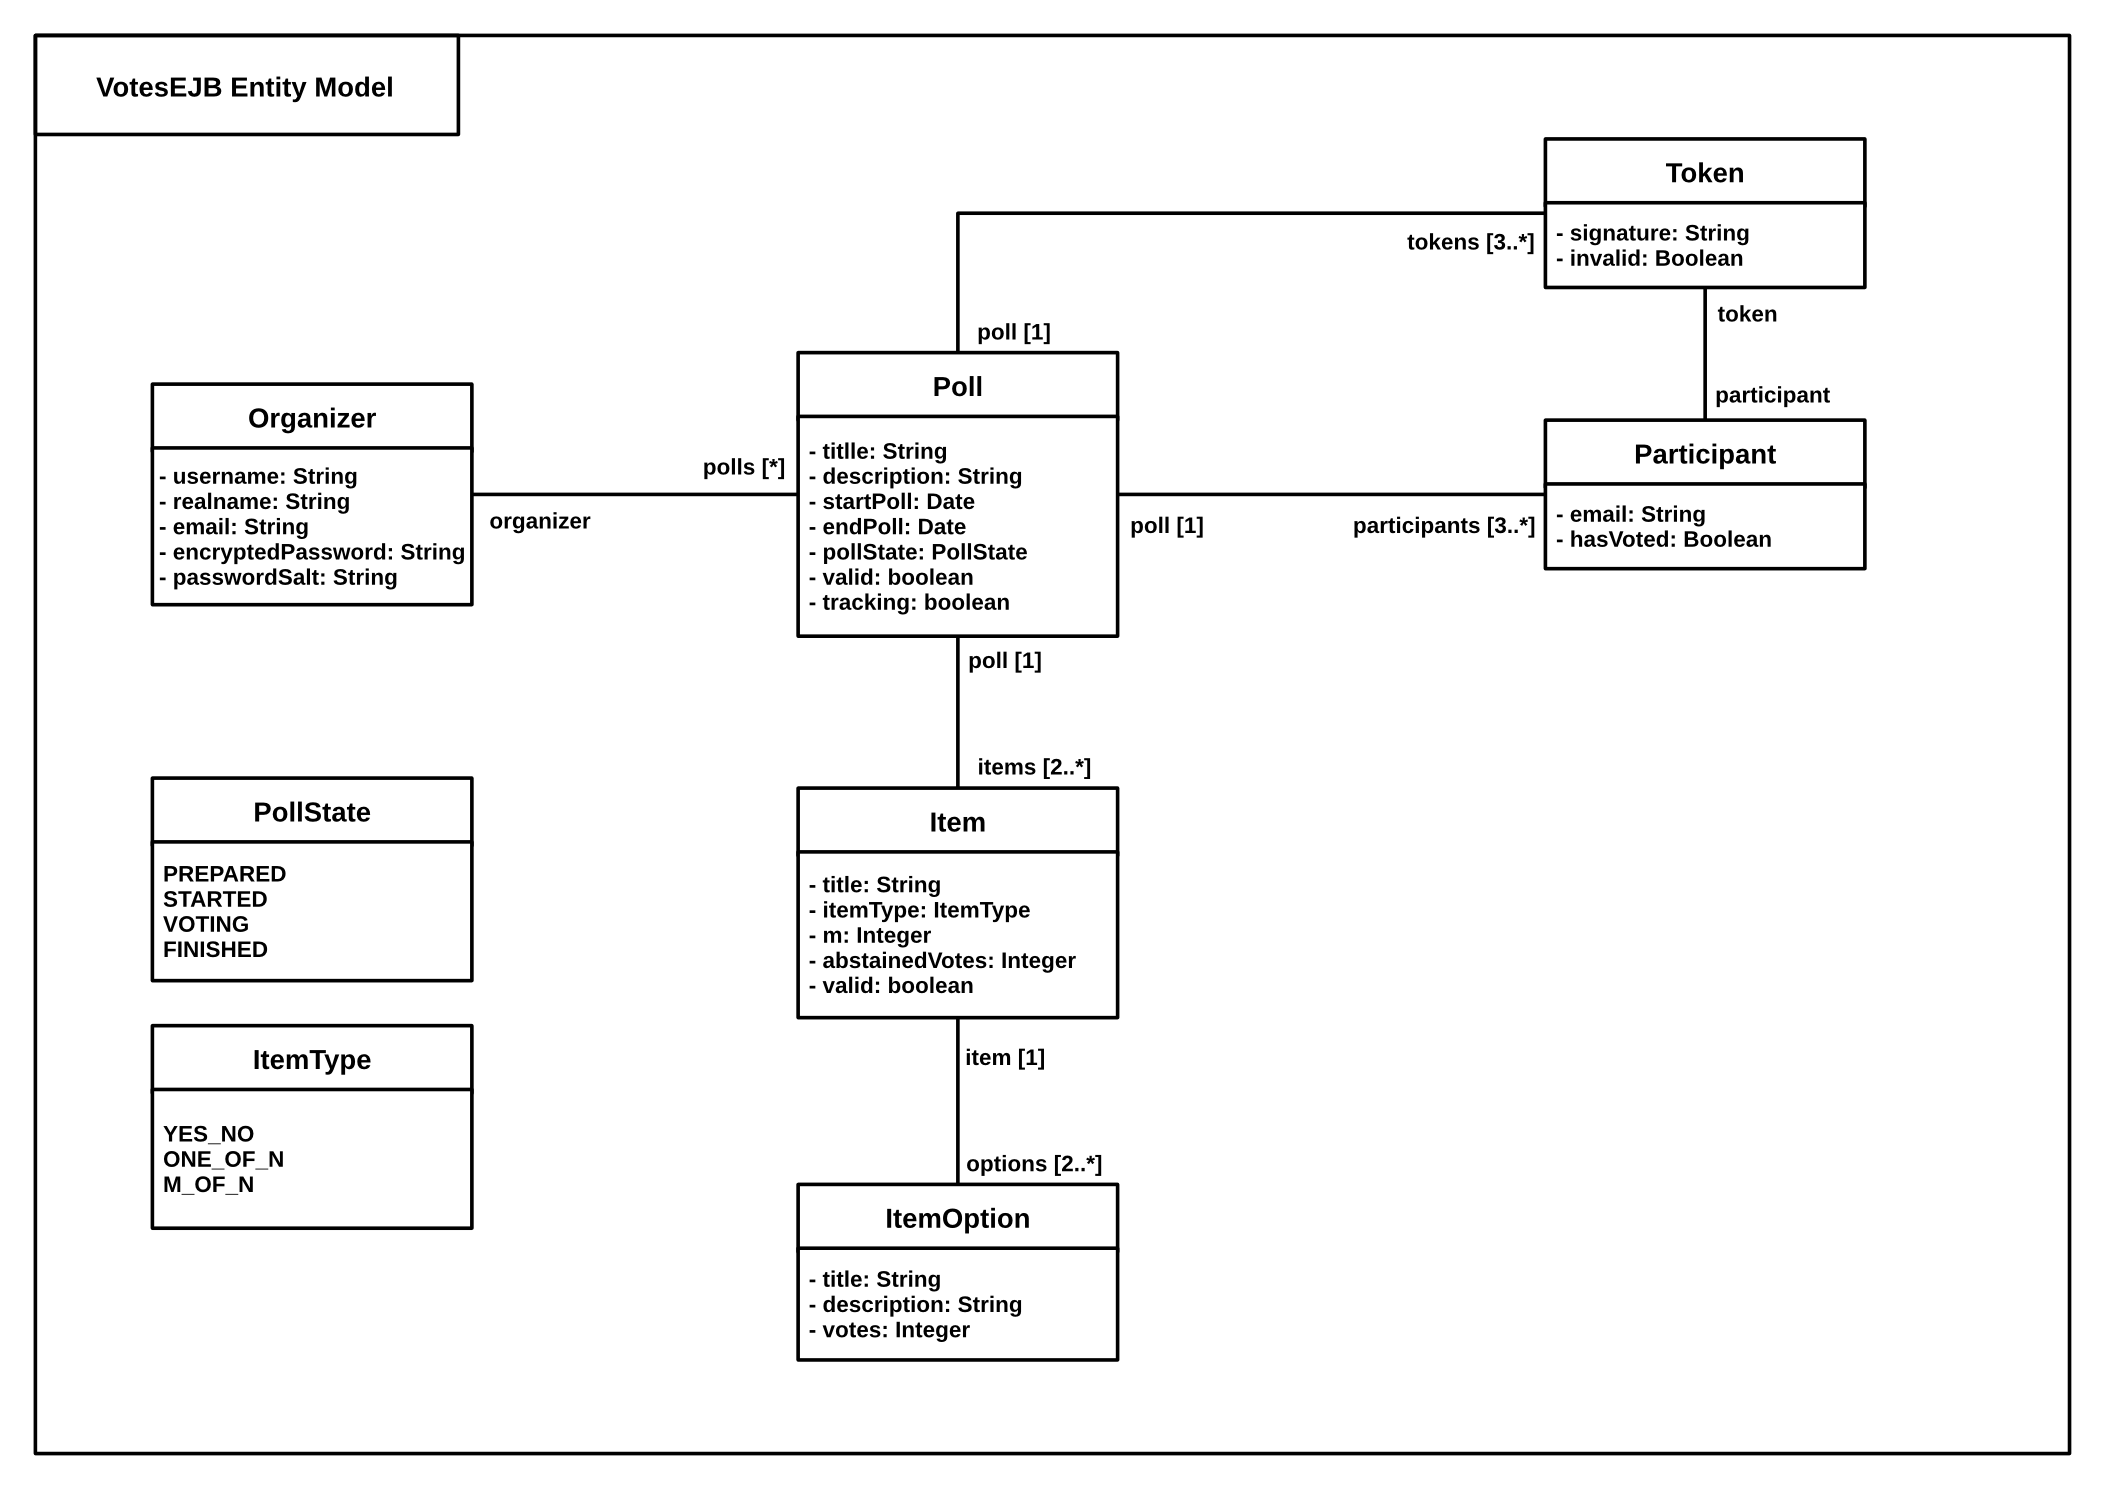
\includegraphics[width=0.7\textwidth]{png/ejb-model.png}
\caption{VotesEJB: Entity Model}
\label{figure:ejb-model}
\end{figure}

\begin{itemize}

\item
Polls and Items have flag, which determines if they are valid.

\item
Items have a counter, which counts abstentions.

\item
ItemOptions have a counter, which counts the number of participants that have selected that said option.

\item
Tokens can be invalidated.

\item
Organizers also store a salt to strengthen password hashes.

\end{itemize}



\paragraph{Anonymity:}
The criterion of utmost importance for a voting system's quality is the degree of assured anonymity.
That means, at no point it must be possible to link a participant to his or hers voting decision.
Therefore certain restriction have been made:
\begin{itemize}

\item
Polls with less than three participants cannot be asserted anonymous, so poll has to have at least three participants.

\item
Although the voting system records which participant has voted for administrative purposes, his or hers exact vote remains unknown to the data structure.
This is ensured by numeric option counters, which increase if a participant has selected an option.

\item
Token signatures act as ballots, which allow a participant to view polls and submit a vote. 
Such signatures must be hard to forge.
To assure this quality, signatures are type 4 UUIDs generated by \texttt{UUID.randomUUID()}\footnote{\url{http://docs.oracle.com/javase/7/docs/api/java/util/UUID.html}}.

\end{itemize}


\paragraph{Security:}
Another issue of importance is reflected by the domain model is the authentication of organizers.
To ensure that only the creators of polls can access their settings, organizer passwords cannot be stored in clear text.
In order to secure the database against attacks, we facilitate the common technique of salted hashes to store passwords.
A password is stored as SHA-256 hash of its concatenation with a type 4 UUID salt.
The salt is stored alongside.


\subsubsection{Votes Entity Persistence}
\label{subsubsec:votes-entity-persistence}
The Java Persistence API (JPA) used by JavaEE Web Applications follow a persistence strategy, which maps entity classes to database tables.
That means for each entity in the domain model exists a corresponding table.
However, to ensure the uniqueness of row tuples, entities need to have an \texttt{id} property, which is missing in figure \ref{figure:ejb-model}.
Entities of the votes domain model inherit such a property from the class AbstractEntity, depicted in figure \ref{figure:ejb-abstract-entity}.

\begin{figure}[h]
\centering
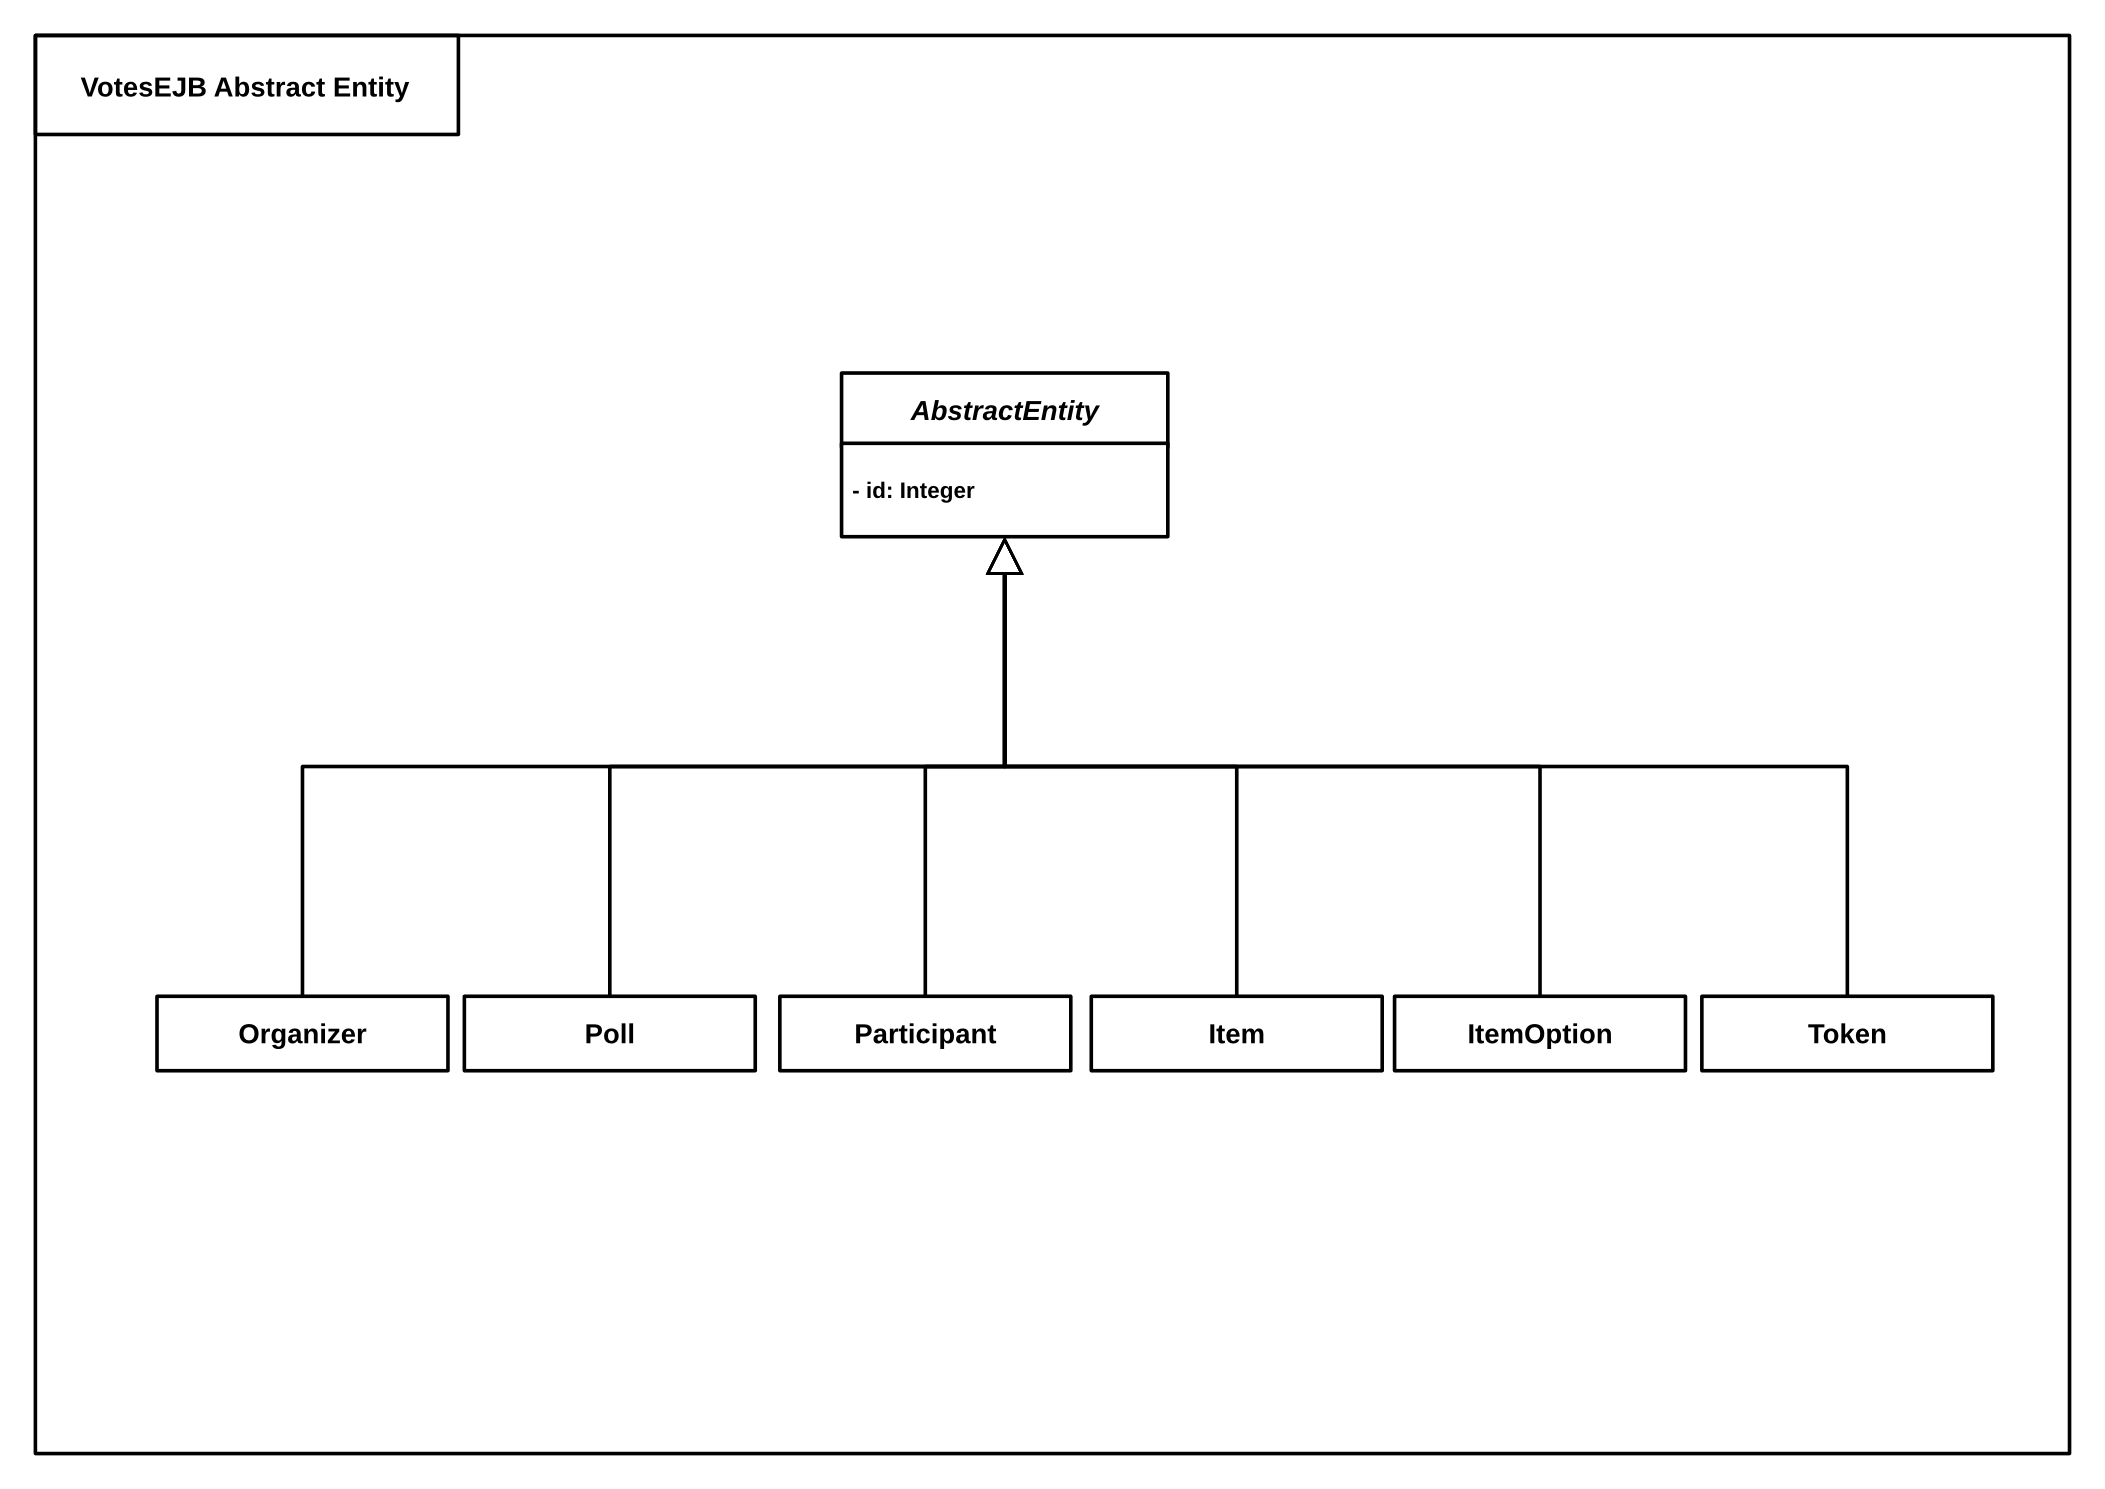
\includegraphics[width=0.7\textwidth]{png/ejb-abstract-entity.png}
\caption{VotesEJB: Abstract Entity}
\label{figure:ejb-abstract-entity}
\end{figure}

Moreover, JPA encourages to use the \textit{Data Mapper}\footnote{\url{http://martinfowler.com/eaaCatalog/dataMapper.html}} pattern to handle persistence operations.
This pattern is exemplified in figure \ref{figure:ejb-data-mapper}, which shows the Poll entity class and its corresponding data mapper PollAccess.

\begin{figure}[h]
\centering
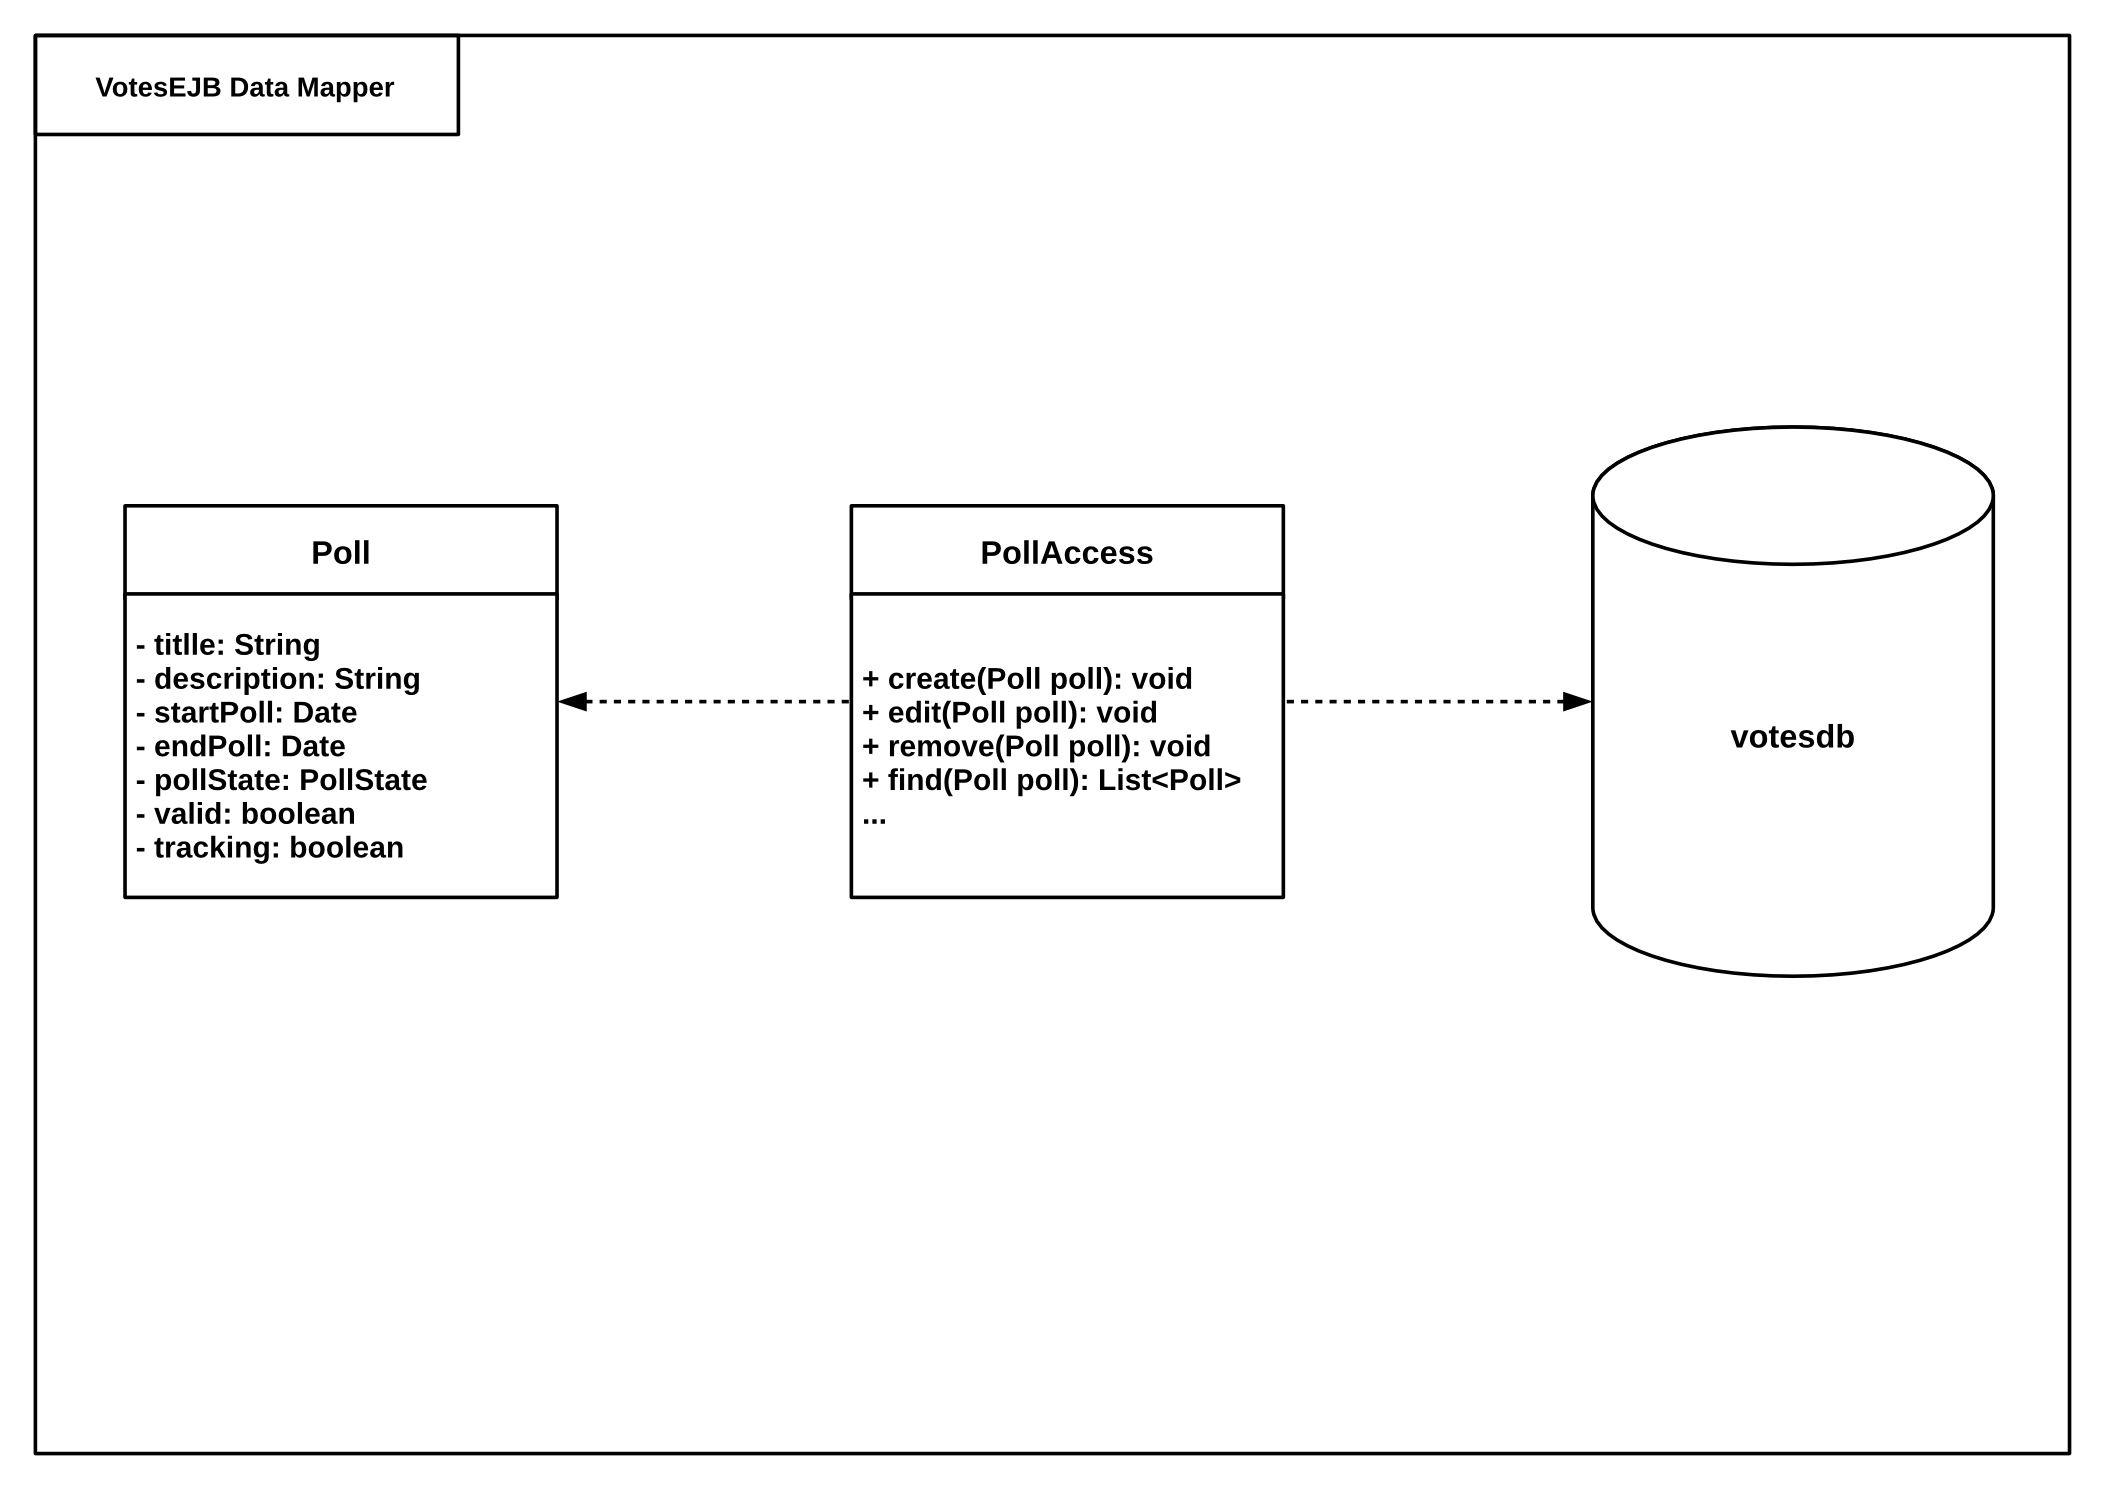
\includegraphics[width=0.7\textwidth]{png/ejb-data-mapper.png}
\caption{VotesEJB: Data Mapper}
\label{figure:ejb-data-mapper}
\end{figure}

Each entity of the votes domain model has its own data mapper handling creation, reading, update and deletion of instances in the database.
Thus, this pattern decouples persistence structure from persistence behaviour. 
Mappers or Data Access Objects are also enhanced to do more complex database operations.

\subsubsection{The Votes Business Model}
\label{subsubsec:the-votes-business-model}
Besides the CRUD operations of the persistence layer, the Votes-System has scarcely any business logic.
One notable exception is the transition of poll states depicted in figure \ref{figure:poll-states}.

\begin{figure}[h]
\centering
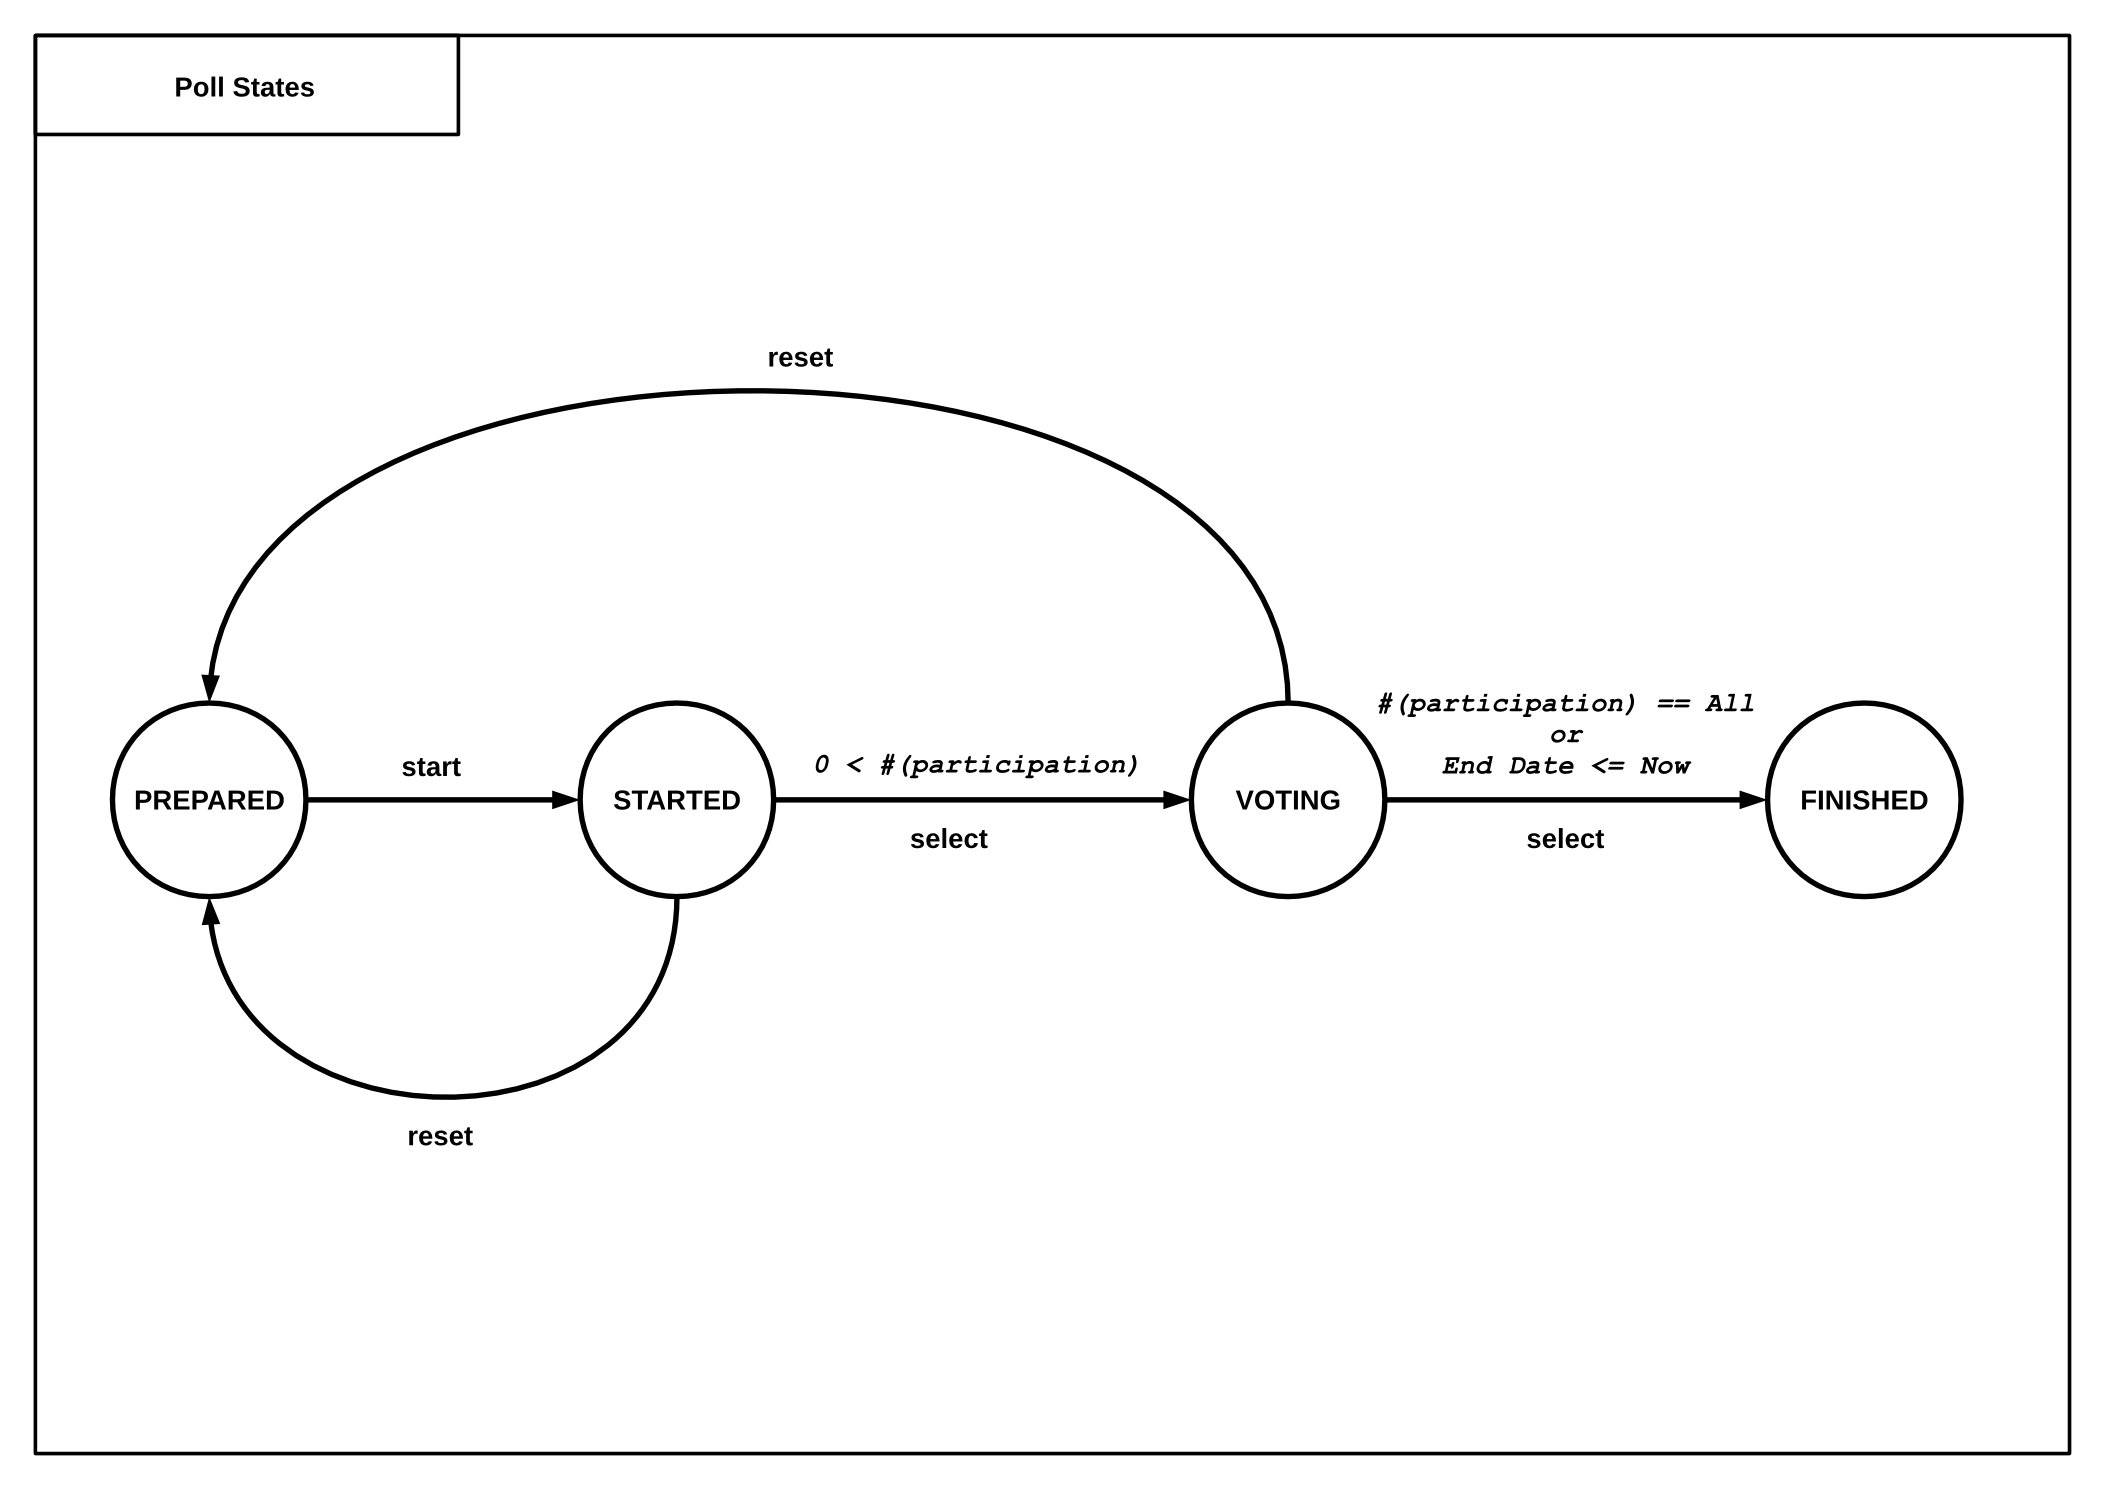
\includegraphics[width=0.7\textwidth]{png/poll-states.png}
\caption{VotesEJB: Poll States}
\label{figure:poll-states}
\end{figure}

Poll states are frequently updated when either an organizer or participant access a certain poll.
Per default, a poll is created in state \texttt{PREPARED}.
If its organizer actively starts the poll, the state changes to \texttt{STARTED}.
This will trigger the sending of notification mails to all participants.
As soon as the first participant has submitted his or her vote the poll state changes to \texttt{VOTING}.
In either poll state \texttt{STARTED} or \texttt{VOTING} the organizer can reset the poll.
However, this will result in the deletion of all submitted votes so far.
When all participants have submitted their votes or the poll period is expired, the poll state changes to \texttt{FINISHED}.
This is the final state of poll.
If this state is reached, no further modification is possible.

\begin{figure}[h]
\centering
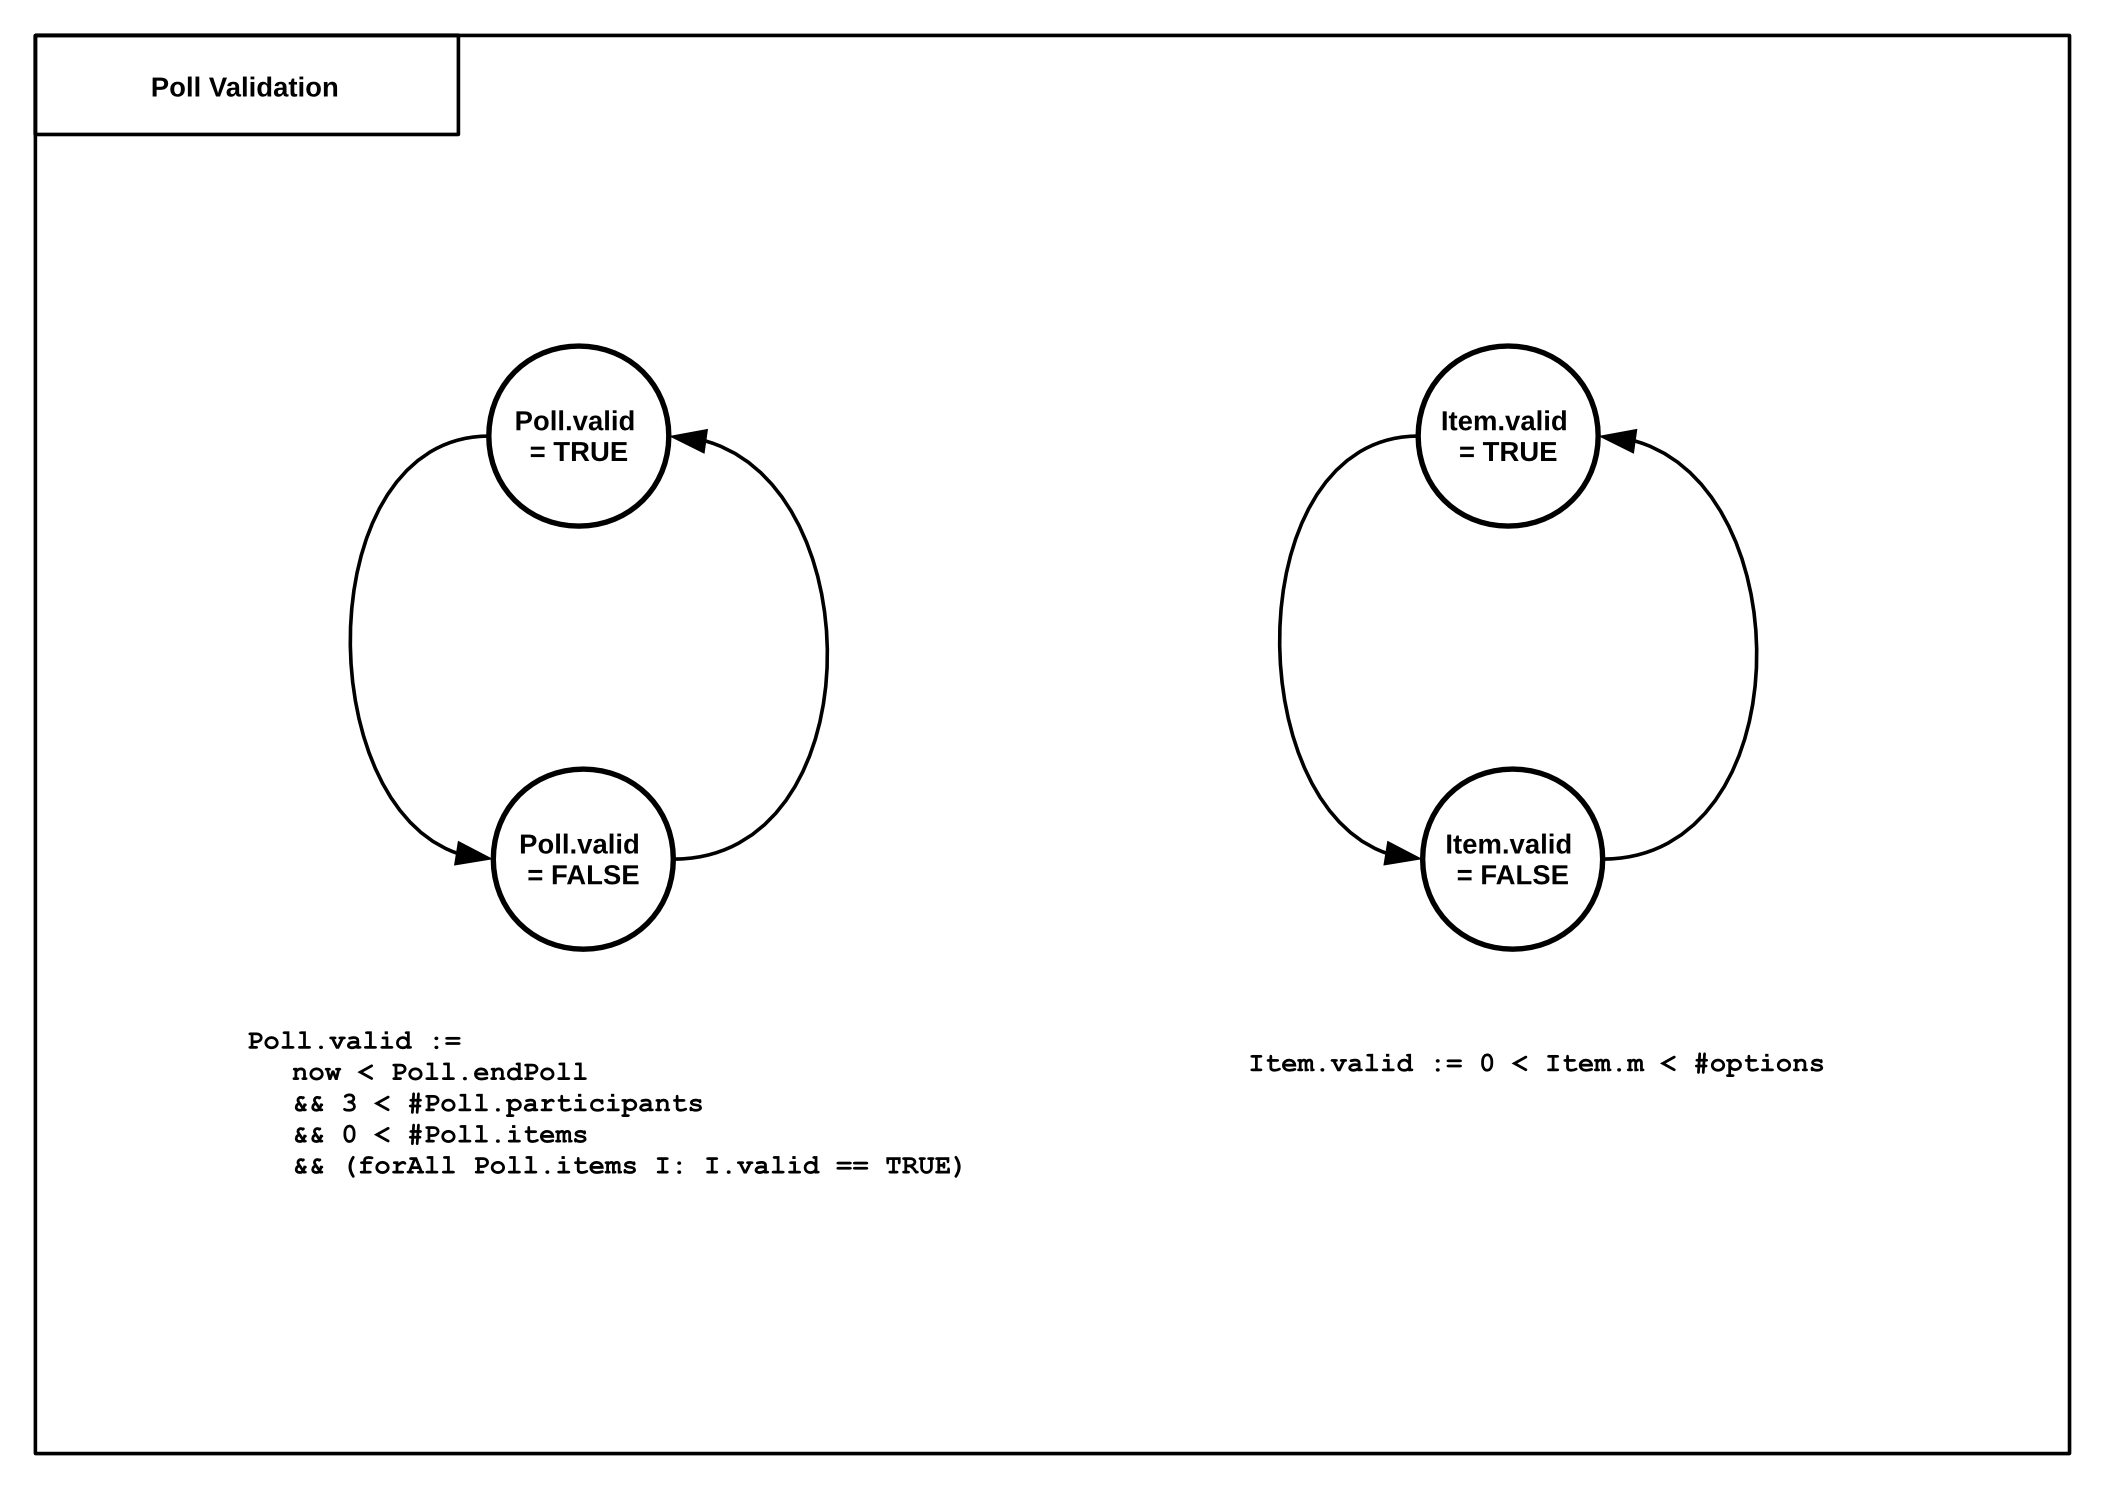
\includegraphics[width=0.7\textwidth]{png/poll-validation.png}
\caption{VotesEJB: Poll Validation}
\label{figure:poll-validation}
\end{figure}

Another notable exception is the validation of polls, depicted in figure \ref{figure:poll-validation}.
Like the poll state, the poll valid flag is frequently updated when a poll is accessed.
Poll validation is one mean to ensure anonymity as only valid polls can be started.
For instance, a poll cannot be valid if less than three participants are defined.

However, such business operations are still closely related to CRUD.
So they are no additional business classes or packages besides the EJB facade, which is described in the following section.

\subsubsection{The VotesEJB Facade}
\label{subsubsec:the-votesejb-facade}
JavaEE Web Applications also encourage the use of the \textit{Facade}\footnote{\url{http://en.wikipedia.org/wiki/Facade_pattern}} pattern.
Facades in general are used to hide complexity by only making the relevant features available to the outside.
The facade of the VotesEJB module called \texttt{VotesLogic} is exemplified in figure \ref{figure:ejb-facade}.

\begin{figure}[h]
\centering
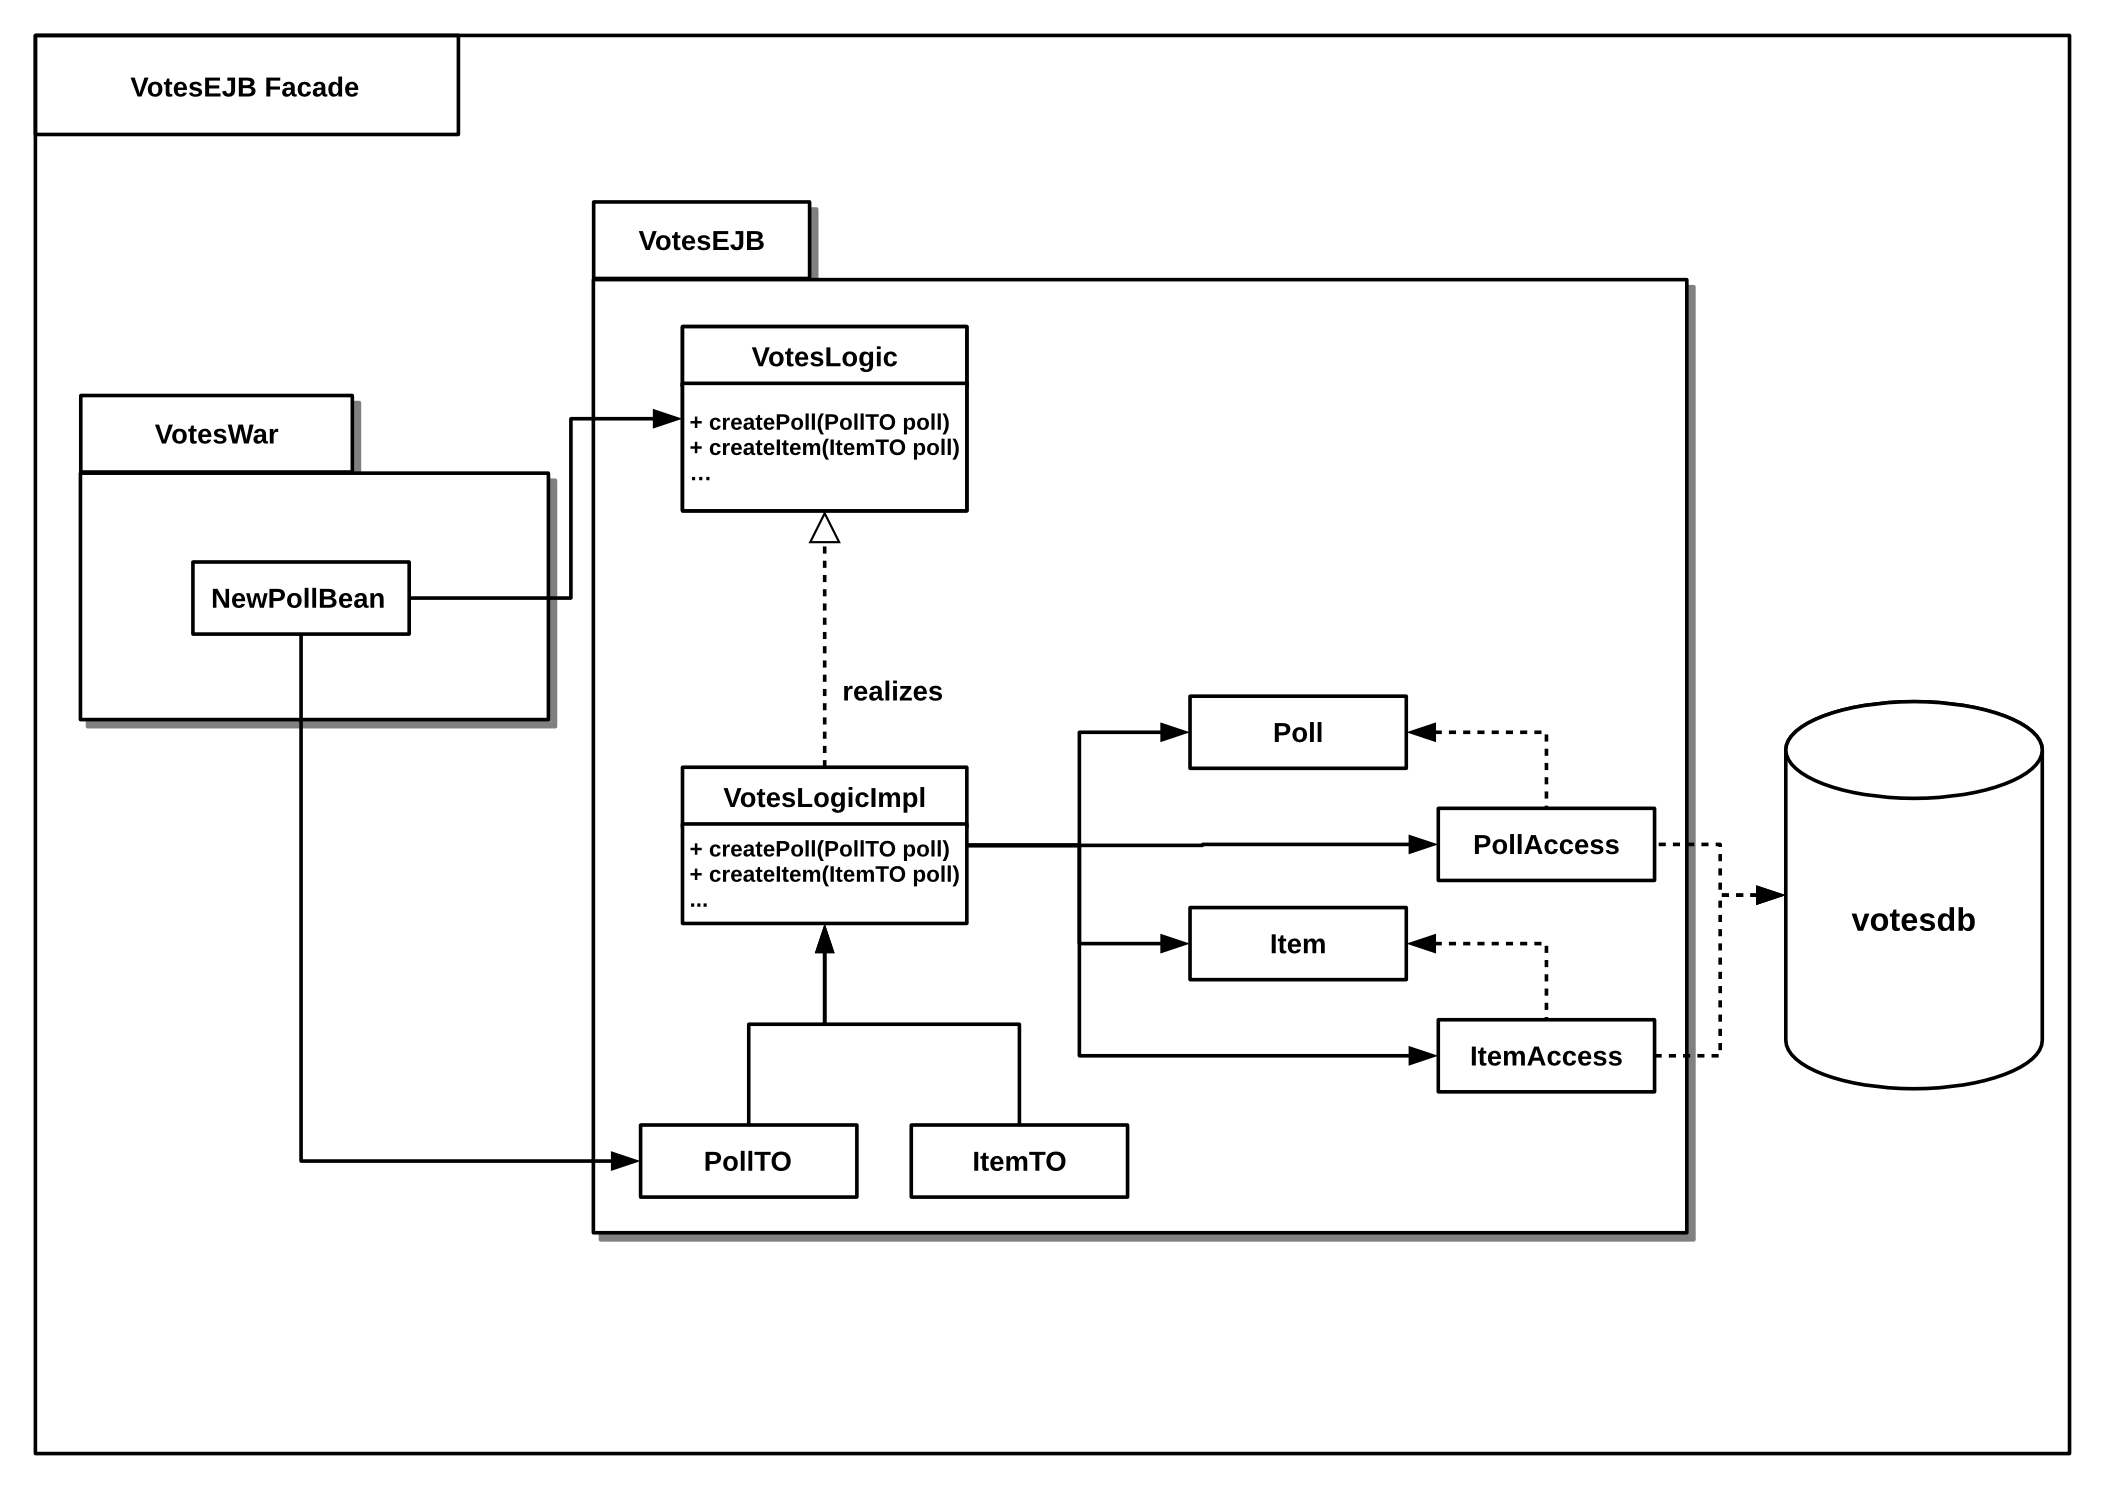
\includegraphics[width=0.7\textwidth]{png/ejb-facade.png}
\caption{VotesEJB: Facade}
\label{figure:ejb-facade}
\end{figure}

The facade is used to handle communication between the VotesEJB and VotesWar modules.
Therefore, the class \texttt{VotesLogicImpl} is injected into beans of VotesWar.
The votes facade provides means to create, read, update and delete entities, and additional business logic methods such as poll validation and user authentication.
Figure \ref{figure:ejb-facade} also shows, that the facade internally uses the data mapper pattern described in section §\ref{subsubsec:votes-entity-persistence}.

Because the VotesEJB and VotesWar modules are instantiated separately, the communication is handled through \textit{Data Transfer Objects}\footnote{\url{http://martinfowler.com/eaaCatalog/dataTransferObject.html}} like \texttt{PollTO} instead of entity objects.
Such transfer objects exactly mirror the structure of entities, but provide a more lightweight form of serialization than entity objects as they do not contain additional mutators.



\subsection{VotesWar Architecture}
JavaEE Web Applications package presentation and user interface logic into WAR modules.
Votes makes use of the JavaServer Faces\footnote{\url{https://javaserverfaces.java.net/}} API (JSF) to create user interface components and their interactions.
In order to create a common look and feel, we use Twitter Bootstrap\footnote{\url{http://getbootstrap.com/}}.
Result charts a created by the Highcharts\footnote{\url{http://www.highcharts.com/}} API.
The outline of votes web pages is depicted in figure \ref{figure:web-directory-outline}.

\begin{figure}[h]
\centering
\begin{minipage}[t]{3cm}
\scriptsize
\begin{verbatim}
\resources
    \bootstrap
    \highcarts
    \jquery
    \votes
        \css
        \img
        \jsf
            ...
            \login.xhtml
            \navbar.xhtml
            ...
\edit-item.xhtml
\edit-poll.xhtml
\my-polls.xhtml
\new-poll.xhtml
\poll.xhtml
\register.xhtml
\result.xhtml
\end{verbatim}
\end{minipage}
\caption{VotesWar: Web Pages Outline}
\label{figure:web-directory-outline}
\end{figure}

All top level XHTML files are accessible through navigation.
Additional resources are packaged into the \texttt{resources} directory.
Note that resources proprietary to votes also contain a \texttt{jsf} directory, containing reusable components, such as a login page or a navbar component.
The login page is only shown if needed to keep the web page as RESTful as possible.

JSF does not enforce any particular pattern as any bean is globally available inside the XHTML template notation.
However, we try to keep a 1:1-mapping between a backing bean and its corresponding web page if possible.
For instance, there is a file \texttt{NewPollBean} corresponding to the page \texttt{new-poll.xhtml}.
Exceptions are made for login handling. 
User information provided by a \texttt{UserBean} is used be various components.

Besides organizer registration, the votes web module handles two kinds of sessions.
That is: organizer sessions, which are used to administer polls.
And participation sessions, which handle the voting interactions of participants.
Both sessions are described in more detail by the following sections.



\subsubsection{Organizer Sessions}
Organizer Sessions are used to create new polls or edit existing polls and their items.
Figure \ref{figure:web-organizer-navigation-graph} depicts the possible navigation between all web pages associated with this session. 

\begin{figure}[h]
\centering
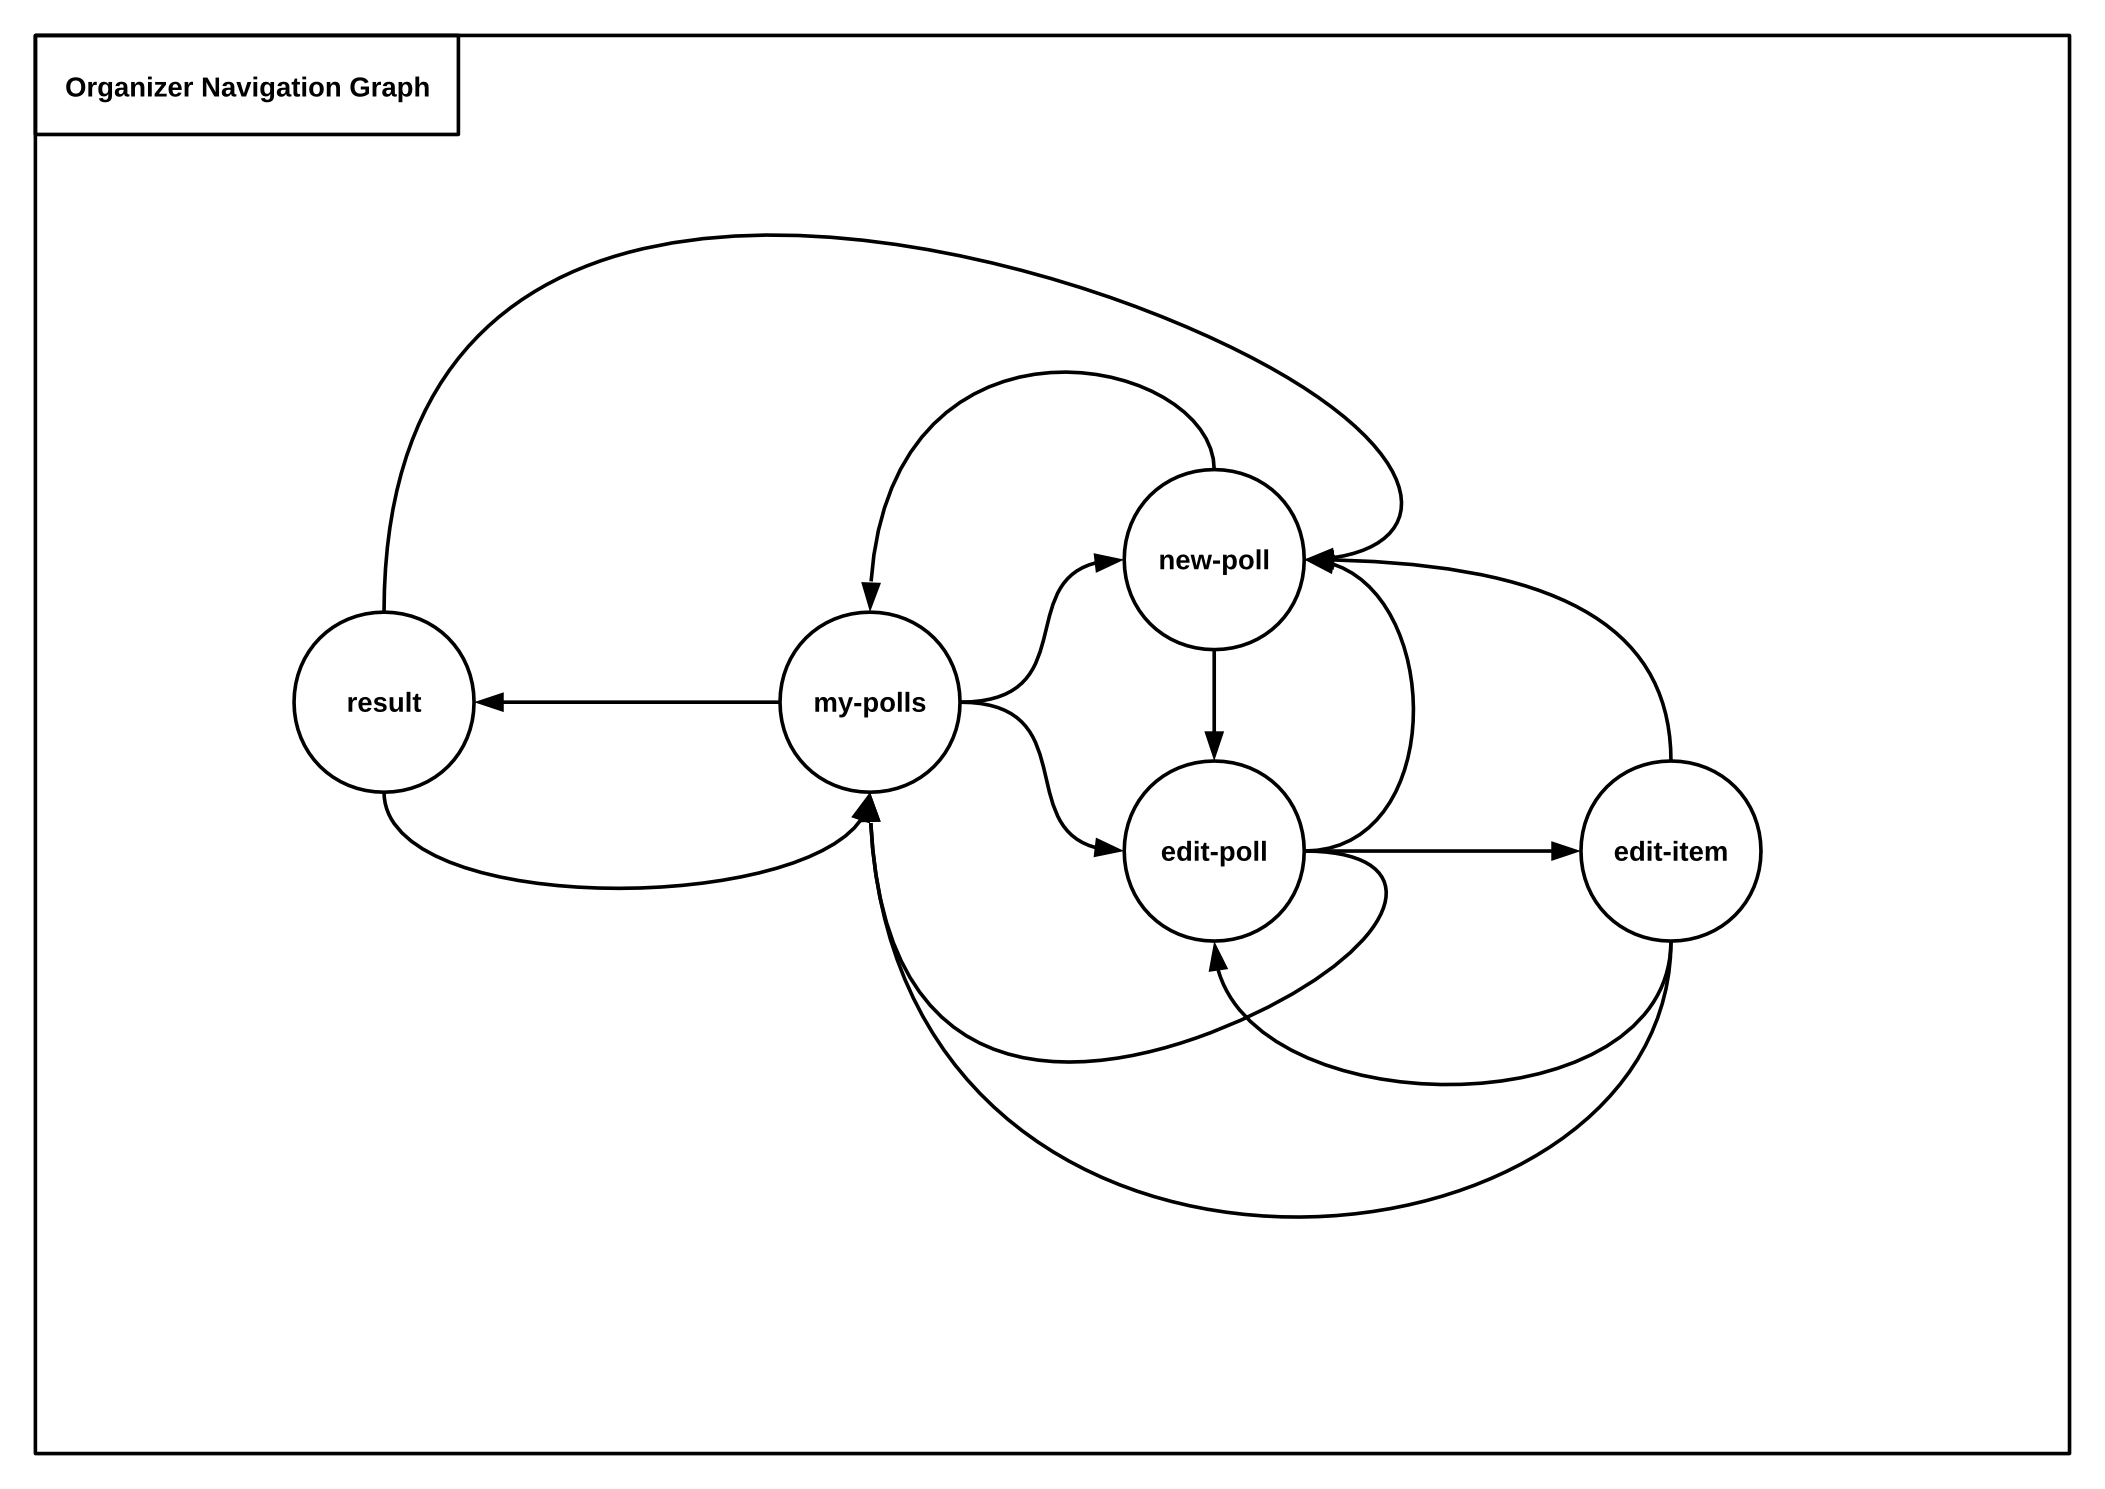
\includegraphics[width=0.7\textwidth]{png/web-organizer-navigation-graph.png}
\caption{VotesWar: Organizer Navigation Graph}
\label{figure:web-organizer-navigation-graph}
\end{figure}

After login, an organizer usually starts at the \texttt{my-poll} page, which shows a table of all polls he or she has created and their current status.
From this page on, it is possible to either create a new poll or edit an existing one.
The pages \texttt{my-polls} and \texttt{new-poll} are available from every other page, because of navigation components.
After an organizer creates a new poll on the \texttt{new-poll} page he gets redirected to the \texttt{edit-poll} page of the same poll.
There he or she can edit the properties of a poll (Title, End-Date, etc.) and add new items or participants. 
By clicking on links of items an organizer navigates to the corresponding \texttt{edit-item} page.
After a poll is finished, it is also possible to navigate to the \texttt{result} page of a poll.

Note, because Votes facilitates a RESTful architecture, every page can be used as starting point with a login beforehand.

\subsubsection{Participant Sessions}
Participant Sessions are used by participants to conduct votes.
Figure \ref{figure:web-participation-state-machine} depicts the states of the page a participant sees while participating.
It is implemented following requirements 10. 

\begin{figure}[h]
\centering
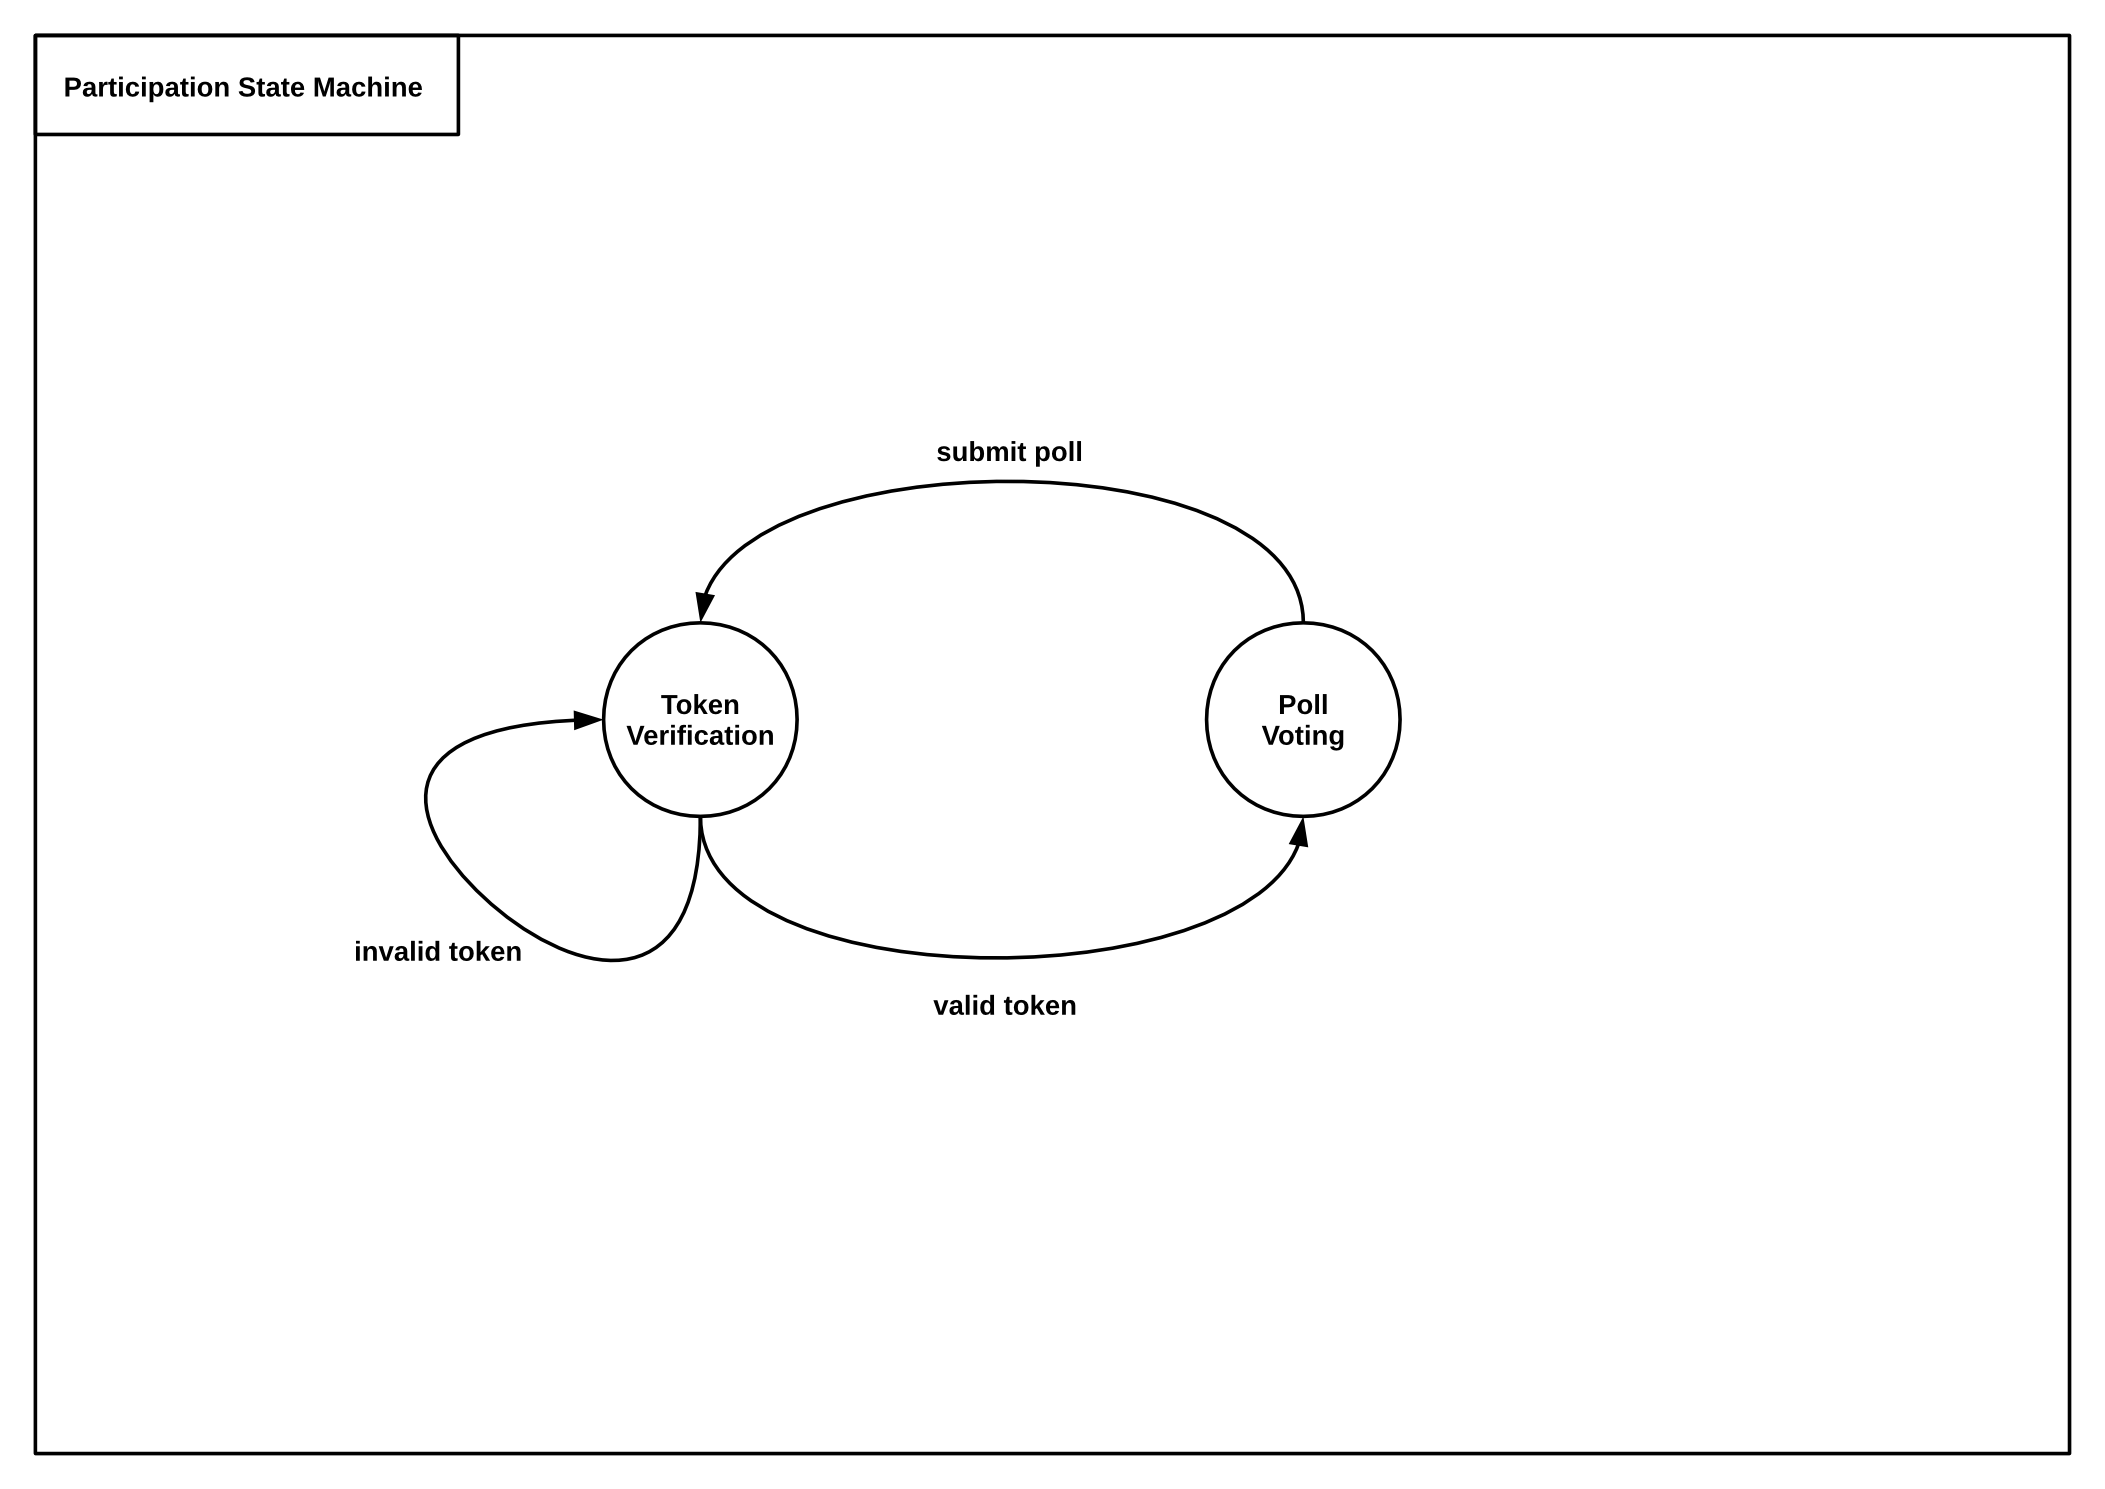
\includegraphics[width=0.7\textwidth]{png/web-participant-state-machine.png}
\caption{VotesWar: Participation State Machine}
\label{figure:web-participation-state-machine}
\end{figure}

At first, a participant asked to verify his or her token as \texttt{Token-Verification}.
If this token is invalid, the participant cannot go onwards.
If the given token is indeed valid, the participant is forwarded to \texttt{Poll-Voting}, where he or she can conduct a vote.
After the participant has submitted the vote, he or she is redirected to the starting point.




\appendix
\section{Installation Guide}
This is a step by step installation guide for the deployment of the Votes-System.
In order to install Votes, we need to open the GlassFish Admin Console in a browser window:

\begin{enumerate}

\item
Make sure GlassFish is started (preferably GlassFish version 4 or higher).

\item
Navigate to \url{http://localhost:4848}.

\end{enumerate}


\subsection{Deploying a New JDBC Connection Pool}

\begin{enumerate}

\item
From \texttt{GlassFish Console - Common Tasks} navigate to \texttt{Create New JDBC Connection Pool}.

\item
Insert the following property values:
\begin{verbatim}
Pool Name:                derby_net_votesdb_rootPool
Resource Type:            javax.sql.DataSource
Database Driver Vendor:   JavaDB
\end{verbatim}

\item
Click \texttt{Next}.

\item 
Set \texttt{Datasource Classname} to: \texttt{org.apache.derby.jdbc.ClientDataSource}

\item
Replace all additional properties with the following (property names are case sensitive):
\begin{verbatim}
User:           root
Password:       password
serverName:     localhost
portNumber:     1527
databaseName:   votesdb
driverClass:    org.apache.derby.jdbc.ClientDriver
URL:            jdbc:derby://localhost:1527/votesdb
\end{verbatim}

\item
Click \texttt{Save}.

\end{enumerate}

\subsection{Deploying a New JDBC Resource}

\begin{enumerate}

\item
From \texttt{GlassFish Console - Common Tasks} navigate to \texttt{Create New JDBC Resource}.

\item
Set \texttt{JNDI Name} to: \texttt{votesdb}

\item
Select \texttt{derby\_net\_votesdb\_rootPool} as \texttt{Pool Name}

\item
Click \texttt{Save}.

\end{enumerate}


\subsection{Deploying a New JavaMail Session}

\begin{enumerate}

\item
sd

\end{enumerate}

\subsection{Deploying Votes}

\begin{enumerate}

\item
From \texttt{GlassFish Console - Common Tasks} navigate to \texttt{Deploy an Application}.

\item
Select the \texttt{Location} of the \texttt{Votes.ear} file.

\item
Click \texttt{OK}.

\end{enumerate}
\section{Manual}
In the following section the most important functionalities of the votes system are summarized.

\subsection{Login}

The Votes login page displayed in figure \ref{F:votes_login} is the entry-point to the system. A direct login is possible by entering an already registered email address an the correct password to the account. If no account has been created the user can sign in by first select \textit{register} in the menu appearing when clicking on the top right button. If the resolution of the browser is high the menu is replaced by buttons in the black top bar. Clicking the \textit{register} button is followed by the registration page. A valid account requires a \textit{Username}, \textit{Realname}, \textit{Email} and \textit{Password}.

\begin{figure}
\centering
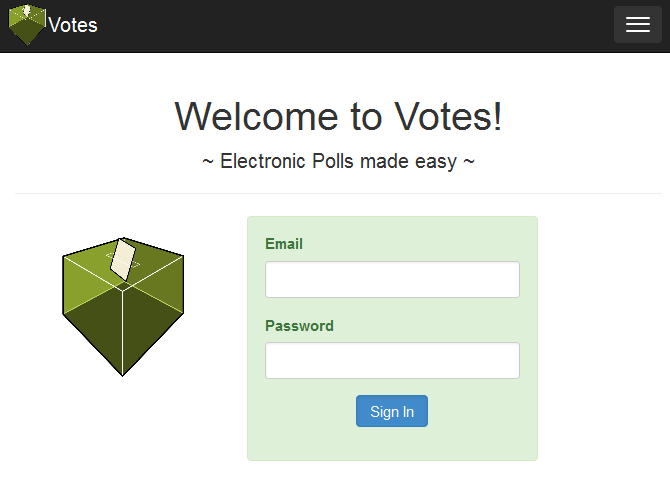
\includegraphics[width=0.4\textwidth]{png/votes_login.png}
\caption{Votes login page}
\label{F:votes_login}
\end{figure}

\subsection{Browse my Polls}
When logged in the \textit{My Polls} page, displayed in figure \ref{F:browse_my_polls}, appears. Here all polls and some poll properties can be viewed on one single page. For informations that go deeper into the Polls data the Poll has to be clicked. The table displays Poll name, state and results. The results can be viewed only when available.

\begin{figure}
\centering
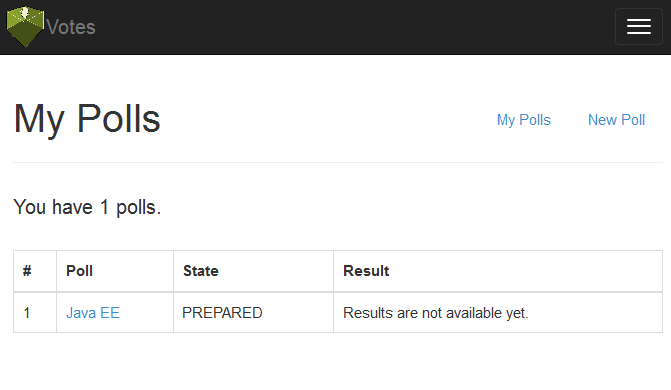
\includegraphics[width=0.4\textwidth]{png/browse_my_polls.png}
\caption{Votes login page}
\label{F:browse_my_polls}
\end{figure}



\subsection{Create and edit Polls}


% Bibliography
%%%%%%%%%%%%%%%%%%%%%%%%%%%%%%%%%%%%%%%%%%%%%%%%%%%%%%%%%%%
{
	\footnotesize
	\bibliography{handbook}
	\bibliographystyle{abbrv}
}

\end{document}